\documentclass[]{elsarticle} %review=doublespace preprint=single 5p=2 column
%%% Begin My package additions %%%%%%%%%%%%%%%%%%%
\usepackage[hyphens]{url}

  \journal{Journal of Transport \& Health} % Sets Journal name


\usepackage{lineno} % add
  \linenumbers % turns line numbering on
\providecommand{\tightlist}{%
  \setlength{\itemsep}{0pt}\setlength{\parskip}{0pt}}

\usepackage{graphicx}
\usepackage{booktabs} % book-quality tables
%%%%%%%%%%%%%%%% end my additions to header

\usepackage[T1]{fontenc}
\usepackage{lmodern}
\usepackage{amssymb,amsmath}
\usepackage{ifxetex,ifluatex}
\usepackage{fixltx2e} % provides \textsubscript
% use upquote if available, for straight quotes in verbatim environments
\IfFileExists{upquote.sty}{\usepackage{upquote}}{}
\ifnum 0\ifxetex 1\fi\ifluatex 1\fi=0 % if pdftex
  \usepackage[utf8]{inputenc}
\else % if luatex or xelatex
  \usepackage{fontspec}
  \ifxetex
    \usepackage{xltxtra,xunicode}
  \fi
  \defaultfontfeatures{Mapping=tex-text,Scale=MatchLowercase}
  \newcommand{\euro}{€}
\fi
% use microtype if available
\IfFileExists{microtype.sty}{\usepackage{microtype}}{}
\usepackage[margin=2cm]{geometry}
\bibliographystyle{elsarticle-harv}
\ifxetex
  \usepackage[setpagesize=false, % page size defined by xetex
              unicode=false, % unicode breaks when used with xetex
              xetex]{hyperref}
\else
  \usepackage[unicode=true]{hyperref}
\fi
\hypersetup{breaklinks=true,
            bookmarks=true,
            pdfauthor={},
            pdftitle={A comparison of objective attributes and cyclists' perceptions along cycling routes in a Canadian developing cycling city},
            colorlinks=false,
            urlcolor=blue,
            linkcolor=magenta,
            pdfborder={0 0 0}}
\urlstyle{same}  % don't use monospace font for urls

\setcounter{secnumdepth}{5}
% Pandoc toggle for numbering sections (defaults to be off)

% Pandoc citation processing

% Pandoc header
\usepackage{setspace}\doublespacing
\usepackage[document]{ragged2e}
\setlength\parindent{24pt}
\setlength{\parskip}{0.0pt plus 1.0pt}
\tolerance=1
\emergencystretch=\maxdimen
\hyphenpenalty=10000
\hbadness=10000
\usepackage{booktabs}
\usepackage{longtable}
\usepackage{array}
\usepackage{multirow}
\usepackage{wrapfig}
\usepackage{float}
\usepackage{colortbl}
\usepackage{pdflscape}
\usepackage{tabu}
\usepackage{threeparttable}
\usepackage{threeparttablex}
\usepackage[normalem]{ulem}
\usepackage{makecell}
\usepackage{xcolor}



\begin{document}
\begin{frontmatter}

  \title{A comparison of objective attributes and cyclists' perceptions along
cycling routes in a Canadian developing cycling city}
    \author[Some School]{Author\corref{Corresponding Author}}
   \ead{author1@address.edu} 
    \author[Some Department]{Author 2}
   \ead{author2@address.edu} 
    \author[Some School]{Author 3}
   \ead{author2@address.edu} 
    \author[Another Department]{Author 4}
   \ead{author2@address.edu} 
    \author[Some School]{Author 5}
   \ead{author2@address.edu} 
      \address[Some School]{School of X}
    \address[Some Department]{Department of Y}
    \address[Another Department]{Department of Z}
    
  \begin{abstract}
  
  \end{abstract}
  
 \end{frontmatter}

\textbf{\emph{Background}}: Cycling is known to have many health
benefits. For this reason, transport planners and public health
officials in Canada increasingly aim to encourage cycling for transport.
On- and off-street infrastructure is often implemented to facilitate
cycling and planners rely on a range of tools for informing the design
of the network of facilities. This mixed methods study compares
objectively measured attributes and cyclists' perceptions of the built
environment along inferred cycling routes in Hamilton, Ontario.\\
\textbf{\emph{Methods}}: Environmental audits were conducted along six
cycling routes in Hamilton to document the attributes that might support
or hinder cycling. The routes were inferred based on the output of a
model of cycling flows. Cyclists, 9 male and 5 female, then participated
in semi-structured interviews where they reviewed photos of the routes
and described their perceptions and preferences. Interview data were
analyzed using both inductive and deductive thematic analysis based on
the categories of the audit instrument.\\
\textbf{\emph{Results}}: Cyclists prefer routes that have dedicated
cycling infrastructure, or residential streets with low volumes of
traffic even if they lack infrastructure. They dislike routes with busy
arterial roads or that lack cycling infrastructure. Their experience and
knowledge of cycling in a city transitioning to be more bicycle-friendly
revealed preferences that can help to improve existing infrastructure
and cycling routes, which may also help to reduce barriers for
non-cyclists.\\
\textbf{\emph{Conclusions}}: The use of photos is an innovative and
practical approach to explore perceptions of regular cyclists, which can
be leveraged to inform policies and interventions to make cycling routes
and infrastructure safer and more attractive. Transport planners in
developing cycling cities should pay attention to a broad range of built
environment factors that influence where people choose to cycle.

\newpage

\hypertarget{sec:introduction}{%
\section{Introduction}\label{sec:introduction}}

Many Canadian cities have adopted pro-cycling policies and programs in
recent years to support the uptake of cycling for transport, including a
range of interventions from investments in infrastructure to educational
programs or promotional events (Assunçao-Denis and Tomalty, 2019). Large
population health gains (Celis-Morales et al., 2017) and improved
environmental conditions in urban areas (Zahabi et al., 2016) could be
achieved if cycling became more mainstream. For instance, Raustrop and
Koglin (2019) estimated that if nearly half of the residents in Scania
county, Sweden cycled to work, almost 20 percent would meet physical
activity guidelines from utilitarian travel alone. The challenge,
however, is how to successfully transition from commonly car-centric
North American cities, to bicycle-friendly cities with larger shares of
active travel.

Active travelers seem to derive intrinsic value from their travel
experience (Whalen et al., 2013). Moreover, travelers also tend to
associate values such as freedom, enjoyment, and happiness with active
travel, even if their regular mode of travel is not active (Mella Lira
and Paez, 2021). However, to convince people to cycle it is also
necessary to create social and built environments that are
bicycle-friendly. Short distances are ideal for cycle trips, which makes
compact mixed-used areas attractive for cycling (Handy, 2020; Pucher and
Buehler, 2008). Streets with slow traffic and traffic calming devices
can also encourage people to use the bicycle for transport (Mertens et
al., 2017). Other features such as adequate lighting and greenery have
been found to support or motivate cycling (Winters et al., 2011), in
addition to increased address and street density (Gao et al., 2018).
Furthermore, cycling experts from both The Netherlands and New Zealand
agree that cycling infrastructure is a universal prerequisite in
countries with an established culture of cycling for transport and in
countries with low levels of cycling (Adam et al., 2020).

Likely for this reason, cities where cycling is less mainstream have
started building infrastructure to encourage more cycling. The case of
Seville, Spain is a great example of the success that can be achieved by
implementing a network of connected facilities at a rapid pace (Marqués
et al., 2015). Revealed and stated preference studies have been further
informative about the types of environments that cyclists prefer and
have reinforced that cycling infrastructure is fundamentally important.
Using global positioning system (GPS) data, several studies have found
that cyclists travel routes that have on-street and off-path cycling
facilities and streets with low volumes of traffic (Broach et al., 2012;
Dill, 2009; Lu et al., 2018; Misra and Watkins, 2018; Scott et al.,
2021). Stated preference studies also indicate that cyclists dislike
mixing with traffic and prefer dedicated infrastructure (\emph{inter
alia}, see Clark et al., 2019; Caulfield et al., 2012; Stinson and Bhat,
2003; Veillette et al., 2019; Winters et al., 2011).

Cities with low but growing levels of cycling have been called
``developing cycling cities'' (Liu et al., 2020), ``low cycling
maturity'' cities (Félix et al., 2019), ``emerging cycling cultures''
(Clark et al., 2019), or ``starter cycling cities'' (Meireles and
Ribeiro, 2020). People who currently cycle in these settings are in the
unique position of observing and experiencing how the city changes over
time to become more bicycle-friendly. Their experiences can highlight
the extent to which a city's current efforts support or hinder cycling.
A few studies in developing cycling cities have found a similarity in
route preferences and barriers to cycling between cyclists and
non-cyclists (see Félix et al., 2019; Clark et al., 2019; Winters and
Teschke, 2010) which also suggests that the perspectives of regular
cyclists may also be informative about what could be improved to
encourage more people to cycle.

A variety of qualitative methods that examine the experience and
perceptions of cycling in such settings can help to centre the cycling
experience in route and infrastructure design. For example, interviews
or mapping exercises (see Manton et al., 2016; Marquart et al., 2020)
and ride-alongs (van Duppen and Spierings, 2013) may shed more light on
reasons for where people cycle and how cycling is experienced. Other
methods that hold promise for cycling research are photovoice and photo
elicitation, techniques that have been used to explore the link between
transportation and well-being (Guell and Ogilvie, 2015; Ward et al.,
2015) and perceptions of the built environment (Alexander, 2013;
Bornioli et al., 2018). These approaches involve the use of images or
photographs in qualitative interviews to evoke memories, feelings, and
experiences about a research phenomenon (Harper, 2002). Photo
elicitation is well-suited for prompting discussion and developing a
comprehensive description of cycling issues, and builds upon the use of
photos in stated preference surveys (see Clark et al., 2019) by enabling
participants to recall and share perceptions or experiences that
influence travel preferences. Environmental audits can also be a useful
tool to document how the built environment supports active travel
(Moudon and Lee, 2003), and have been used in studies to explore
walkability. Qualitative evidence captured from photo elicitation or
interviews can thus complement objective assessments of the physical
environment studied through methods like environmental audits or GIS
(see Lee and Dean, 2018), and has the potential to inform mobile
applications or platforms to induce cycling (see Meireles and Ribeiro,
2020).

In this paper, a sequential explanatory mixed methods approach compares
objectively measured attributes and cyclists' perceptions of the built
environment along inferred cycling routes in Hamilton, Ontario. This
project explored the influence of the built environment on cycling in a
mid-sized Canadian city with low but growing cycling levels. We
previously estimated a spatial interaction model to investigate the
correlates of cycling in Hamilton and found that the \emph{quietest}
distance route between cycling trip zones of origin and destination
inferred by \emph{CycleStreets} best explained cyclist travel in
Hamilton and led to the most parsimonious model {[}paper submitted to
\emph{Transportation}{]}. Given that the routes were inferred, we did
not know the quality of their built environment or how well they match
where cyclists actually travel in Hamilton. To further explore these
objectives, we audited 6 inferred routes to document attributes that
might influence cycling. We then used photos of the routes, or
photo-journeys, in 14 semi-structured interviews with regular cyclists
to examine their perceptions of the routes.

\hypertarget{sec:methods}{%
\section{Methods, Research Setting, and Materials}\label{sec:methods}}

\hypertarget{research-setting}{%
\subsection{Research Setting}\label{research-setting}}

Hamilton is a mid-sized city located in Canada with a population of
roughly 740,000 according to the 2016 Canadian Census (Statistics
Canada, 2017). The city is relatively flat but is separated by the
Niagara Escarpment, referred to locally as ``the mountain'', which can
be as high as 100m in many places. The rural and suburban parts of the
city are on top of the Escarpment and the lower city and downtown core
are below {[}see Figure 1 for reference{]}. Similar to other Canadian
cities, cycling levels have grown in recent years; the mode share of
cycling for transport doubled from 0.6\% in 2011 to 1.2\% according to
the 2016 \emph{Transportation Tomorrow Survey} (\emph{TTS}) (Data
Management Group, 2018). This voluntary travel survey is conducted every
5 years to collect information about urban travel for commuting purposes
in Southern Ontario (Data Management Group, 2018). Between the 2011 and
2016 surveys, the City of Hamilton implemented a public bicycle share
program (PBSP) and added 85 kilometres of bicycle lanes. Hamilton is the
only mid-sized city in Canada with a PBSP which reflects that the City
has invested a lot of effort in the potential for Hamilton to become a
mid-sized cycling city in North America. As of 2019, approximately 46\%
of the cycling network has been built and approximately 15 to 20 km of
new facilities are added each year. The City's current Cycling Master
Plan states that the goal is to implement all proposed infrastructure by
2029 (City of Hamilton, 2018a), but the City's typical annual investment
in cycling infrastructure falls short of what is needed to meet this
goal. Therefore, it is suggested that Hamilton is a developing cycling
city because it is currently in a state of transition and has growing
cycling levels. The City is at the mid-way point in the development of
its cycle infrastructure network. Other interventions have been
implemented to increase cycling levels, but the cycling culture is still
growing and the network is currently fragmented.

This paper contributes to the growing body of research on cycling and
active travel in mid-sized Canadian cities in recent years (Fischer et
al., 2020; Klicnik and Dogra, 2019; Mayers and Glover, 2020; Winters et
al., 2018). Mid-sized cities in Ontario offer unique opportunities for
future growth and development despite but face existing challenges to
transportation and land use planning (Evergreen, 2017). In the case of
Hamilton, efforts to increase pedestrian and cyclist-friendly spaces are
constrained by the city's efforts in the mid-1900s to prioritize
automobile traffic on arterial roads (Leanage and Filion, 2017). Despite
the legacy of Hamilton's car-oriented streets, building a cycling
network in mid-sized cities is promising because of short trip distances
(Winters et al., 2018), which can make cycling appealing given the
proper investment in supportive infrastructure. Indeed, further analysis
of the 2016 \emph{TTS} revealed that 35\% of all current trips in
Hamilton are 5 km or less (Mitra et al., 2016), which means that these
trips could be cycled. The City of Hamilton also aims to have 15\% of
the mode share be comprised of walking and cycling trips by 2031 (City
of Hamilton, 2018b). In this stage of transition, there is the potential
to incentivize modal shifts that specifically increase opportunities for
physical activity.

\begin{figure}

{\centering 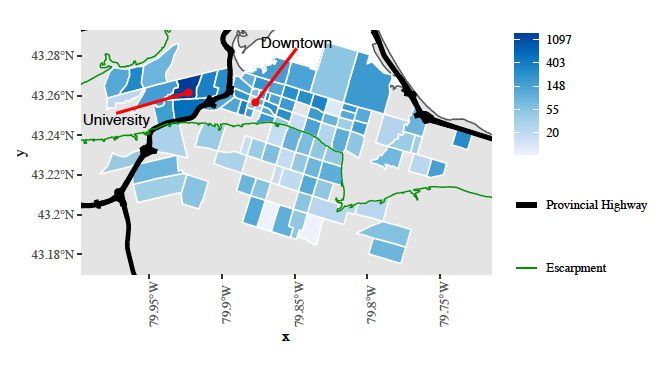
\includegraphics[width=0.65\linewidth]{TAZ-Hamilton} 

}

\caption{The number of cycle trips reported for each traffic analysis zones in the city of Hamilton that produced cycle trips. The number of cycle trips (ranging from more than 1 to over 1097) are shown by the colour gradient. Most cycle trips reported occur around the University.}\label{fig:figure-1}
\end{figure}

\hypertarget{previous-research}{%
\subsection{Previous Research}\label{previous-research}}

In the first phase of this project, {[}paper submitted to
\emph{Transportation}{]}, we used bicycle trip data from the 2016
\emph{TTS} to develop a spatial interaction model that investigated the
built environment correlates of cycling flows in Hamilton. While the
\emph{TTS} is informative about the traffic zones of origin and
destination of cycling trips, it does not reveal the route choice of
respondents. Thanks to the growth in open source resources for
transportation analysis (Lovelace, 2021), a novel feature of this model
was the use of a cycle routing algorithm to infer different types of
cycle routes between zones of origins and destinations (Lovelace and
Lucas-Smith, 2018). The centroid of each traffic analysis zone, the
geographical unit of analysis used by the \emph{TTS}, serves as the
start and end point for these inferred routes. The distance and time of
three different types of routes, characterized as \emph{fastest},
\emph{quietest}, or \emph{balanced} by the \emph{CycleStreets}
algorithm, were used as measures of impedance in the model. Briefly, the
\href{https://cran.r-project.org/web/packages/cyclestreets/index.html}{\texttt{R}
package} states, ``These represent routes taken to minimize time, avoid
traffic, and compromise between the two, respectively'' (Lovelace and
Lucas-Smith, 2018, p. 1). Additional details about the algorithm are
available
\href{https://www.cyclestreets.net/help/journey/howitworks/}{online}.
The model revealed that inferred \emph{quietest} routes that allow
cyclists to minimize distance and interactions with other road users
best explain the pattern of travel by bicycle in Hamilton {[}paper
submitted to \emph{Transportation}{]}. The \emph{quietness} score takes
into account attributes of the road, mainly the presence or absence of
cycle infrastructure. Our findings suggests that cyclists in Hamilton
are seeking out routes that enable them to avoid traffic while
potentially maximizing the use of residential streets over arterial
roads. We then used the model to identify trip flows where there was
more or less cycling than expected (i.e., reported number vs.~predicted
number of cycle trips). The model did not capture any route-level
characteristics beyond the data available for Hamilton through
\emph{OpenStreetMap} that was used by the algorithm. Therefore (see
Moniruzzaman and Páez, 2012), it was hypothesized that more cycling
occurred between zones of origin and destination that were
under-estimated because the inferred routes facilitate cycling (meaning
that there was \emph{more} cycling between the zones than predicted by
the model), for example through the provision of infrastructure.
Conversely, cycling trips may have been over-estimated if routes between
zones of origin and destination are less supportive of cycling (meaning
that there was \emph{less} cycling between zones than predicted by the
model).

\hypertarget{methods}{%
\subsection{Methods}\label{methods}}

\hypertarget{environmental-audits}{%
\subsubsection{Environmental Audits}\label{environmental-audits}}

We conducted environmental audits along 6 inferred routes that were most
substantially over- or under-estimated by the model. The
\emph{Systematic Pedestrian and Cycling Environmental Scan}
(\emph{SPACES})\footnote{\href{https://activelivingresearch.org/sites/activelivingresearch.org/files/SPACES_Audit_Instrument_0.pdf}{SPACES
  Audit Instrument}} (Pikora et al., 2002) was selected because it
documents the presence or absence of observable characteristics that are
potential influences of walking and cycling. The framework describes
four domains of the built environment that influence physical activity:
functional, safety, aesthetic, and destination (Pikora et al., 2003).
The instrument was developed for use along street segments within
neighbourhoods around a residential location. While the cycling trip
flows in Hamilton occur beyond the 400 m neighbourhood range, our unit
of analysis, namely segments of a street, is the same as the
\emph{SPACES Instrument}. The instrument also includes an extensive
range of measurable features that have been identified in the literature
which meet our objective in conducting an exploratory and descriptive
analysis of attributes along the inferred cycling routes. For these
reasons, we determined that the \emph{SPACES Instrument} was suitable
for our purposes. This instrument was also selected because it is
relatively simple to use and developed for research purposes (Moudon and
Lee, 2003). The instrument comes from the field of health and the
factors included in the audit were guided by stakeholder interviews and
a Delphi study (Pikora et al., 2003).

The \emph{SPACES Instrument} was adapted to the local context in
Hamilton. Cycling was the primary focus of this study; accordingly, some
factors that were less influential on cycling, according to the
literature, were removed for ease of data collection. The features that
were removed from the instrument used in this study include:
\emph{permanent path obstructions}, \emph{pedestrian crossing aids},
\emph{surveillance}, \emph{building design}, and \emph{driveway
crossovers}. Other features were combined: all types of maintenance
instead of specific categories, and the types of paths. A broader range
of cycling facilities, buildings, and traffic calming measures that are
found in Hamilton were also added. The modified \emph{SPACES Instrument}
is shown in Appendix A and the Hamilton cycling guide added to the
\emph{SPACES Observation Manual} is found in Appendix B. The first
author and three research assistants conducted the audits during October
and November 2019. The first author was the only auditor who has cycling
experience in Hamilton. Each auditor participated in a training exercise
led by the first author to become familiar with the \emph{SPACES
Instrument} and the \emph{SPACES Observation Manual}\footnote{\href{https://activelivingresearch.org/sites/activelivingresearch.org/files/SPACES_Observation_Manual.pdf}{SPACES
  Observation Manual}} (Pikora et al., 2002), and to standardize the way
in which the audits were carried out. The majority of routes
(\(n = 4/6\)) were audited by a pair of research assistants who filled
out the instrument together. Two routes (\(n = 2/6\)) were audited by
the first author alone. The auditors were instructed to discuss any
disagreements and reach consensus before filling out the instrument.
Once the audits were completed, the features of each route segment were
manually recorded in an Excel sheet by the first author. Any perceived
errors in data collection were reviewed using Google Street View and
were corrected by the first author. A descriptive analysis of each route
was performed to determine the presence and frequency of features along
each route.

\hypertarget{interviews}{%
\subsubsection{Interviews}\label{interviews}}

Following the audits, 14 cyclists in Hamilton were recruited to
participate in a 90-minute semi-structured interview {[}see Table
\ref{tab:demographics} for demographics of participants{]}. We employed
a convenience sampling strategy to recruit participants using posters in
local bike stores and coffee shops in Hamilton and a social media post
on Twitter. A total of 28 people responded to the recruitment notice,
and the first 14 who met the inclusion criteria were recruited to the
study. Inclusion criteria were as follows: age (18 years of age or
older) and regular travel by bicycle for transport in Hamilton. The
latter was defined as cycling for transport at least once per week.

\begin{table}

\caption{\label{tab:unnamed-chunk-1}\label{tab:demographics}Demographics of participants (age, gender, self-reported frequency of cycling, and self-reported confidence level).}
\centering
\fontsize{7}{9}\selectfont
\begin{tabular}[t]{>{}l|llll}
\toprule
Participant & Age & Gender & Frequency & Confidence\\
\midrule
\em{\cellcolor{gray!6}{1}} & \cellcolor{gray!6}{18-24} & \cellcolor{gray!6}{Male} & \cellcolor{gray!6}{Every day} & \cellcolor{gray!6}{Excellent}\\
\em{2} & 25-44 & Male & Multiple times a week & Excellent\\
\em{\cellcolor{gray!6}{3}} & \cellcolor{gray!6}{25-44} & \cellcolor{gray!6}{Female} & \cellcolor{gray!6}{Multiple times a week} & \cellcolor{gray!6}{Excellent}\\
\em{4} & 25-44 & Male & Multiple times a week & Excellent\\
\em{\cellcolor{gray!6}{5}} & \cellcolor{gray!6}{45-64} & \cellcolor{gray!6}{Male} & \cellcolor{gray!6}{Multiple times a week} & \cellcolor{gray!6}{Good}\\
\addlinespace
\em{6} & 45-64 & Male & Every day & Excellent\\
\em{\cellcolor{gray!6}{7}} & \cellcolor{gray!6}{45-64} & \cellcolor{gray!6}{Male} & \cellcolor{gray!6}{Multiple times a week} & \cellcolor{gray!6}{Excellent}\\
\em{8} & 45-64 & Male & Multiple times a week & Good\\
\em{\cellcolor{gray!6}{9}} & \cellcolor{gray!6}{25-44} & \cellcolor{gray!6}{Female} & \cellcolor{gray!6}{Multiple times a week} & \cellcolor{gray!6}{Excellent}\\
\em{10} & 25-44 & Male & Every day & Excellent\\
\addlinespace
\em{\cellcolor{gray!6}{11}} & \cellcolor{gray!6}{25-44} & \cellcolor{gray!6}{Female} & \cellcolor{gray!6}{Multiple times a week} & \cellcolor{gray!6}{Good}\\
\em{12} & 25-44 & Female & Every day & Excellent\\
\em{\cellcolor{gray!6}{13}} & \cellcolor{gray!6}{25-44} & \cellcolor{gray!6}{Male} & \cellcolor{gray!6}{Every day} & \cellcolor{gray!6}{Excellent}\\
\em{14} & 25-44 & Female & Multiple times a week & Excellent\\
\bottomrule
\end{tabular}
\end{table}

The first author conducted the interviews, ranging in time from 60 to 90
minutes, between November 2019 and January 2020 at either the
institution, a local coffee shop, or local library. Participants were
presented with three packages of photos that each contained two routes
(i.e., the first package contained routes \emph{1A} and \emph{1B}; the
second contained routes \emph{2A} and \emph{2B}; and the third contained
routes \emph{3A} and \emph{3B}). Table \ref{tab:routes} provides a
description of the routes. This approach can be considered a form of
photo elicitation (Harper, 2002), whereby images are used to prompt
memory, emotions, and experience of a particular phenomenon (e.g.,
identity, culture, place, etc.). The photos of the routes audited were
taken from Google Street View, using the most recent photos available to
ensure that they matched the current streetscape as much as possible. As
such, the time of day or day of the week that the photos were taken may
not reflect prime cycling times and likely traffic volumes expected at
those times. We used photos to understand how these routes were
perceived or experienced based on cyclists' knowledge or history of
traveling through these spaces. In contrast to photo elicitation, which
typically uses standalone photos of a particular item of interest (e.g.,
infrastructure design or route type), a novel aspect of our approach is
the sequential nature of the photos presented in the interviews.
Therefore, these photo journeys include a more dynamic, temporal element
that allows participants to follow the route, and see and comment on the
changes that they perceive. This enables us to capture both perceptions
of specific attributes of the routes as well as the experiences or
impressions of the journey as a whole.

The first two packages each had one route where cycling was
over-estimated by the original model (i.e., \emph{1A} and \emph{2A}),
and one route where cycling was under-estimated by the original model
(i.e., \emph{1B} and \emph{2B}). The final package had two routes where
cycling was under-estimated (i.e., \emph{3A} and \emph{3B}). The routes
in each package were paired according to their length and number of
segments {[}see Table \ref{tab:routes}{]}. Participants did not know
which routes were over- and under-estimated. The photos for each route
were numbered to make it easier to transcribe and ensure that
participants' comments could be attributed to the appropriate segment.
Segments that were long or that had changing attributes in the same
segment were depicted through multiple photos. Participants were asked
to look through the photos of each route from start to finish and then
to share their perceptions by commenting on what they liked and disliked
about the route. However, some participants preferred to make comments
as they looked through the photos. After commenting on both routes in
one package, participants were asked which route they preferred.
Additional questions were asked if a participant reported having cycled
part of a route or if they described taking a different route than the
one inferred. Other follow-up probing questions were asked to better
understand participants' perceptions or experiences of the route.

The interviews were audio recorded and later transcribed using Temi, an
\href{https://www.temi.com/}{online AI-based transcription software}.
The first author then reviewed and proofread each transcript. The first
author coded all of the interviews and conducted a thematic analysis
using both inductive and deductive approaches (Braun and Clarke, 2006).
Themes were determined by the frequency of codes (Braun and Clarke,
2006), meaning the number of different participants who expressed a
similar like, dislike, or perception for each route. Themes identified
using a deductive approach aligned with the attribute categories from
the \emph{SPACES Instrument}, while other themes were identified using
an inductive approach based on perceptions and experiences that emerged
in the interviews. Themes were identified for each individual route and
not for the collective of six routes.

\hypertarget{ethics}{%
\subsubsection{Ethics}\label{ethics}}

This study was approved by the institution's research ethics board in
September 2019.

\hypertarget{sec:findings}{%
\section{Findings}\label{sec:findings}}

\hypertarget{observable-route-attributes-measured-using-the-spaces-instrument}{%
\subsection{Observable Route Attributes Measured using the SPACES
Instrument}\label{observable-route-attributes-measured-using-the-spaces-instrument}}

A total of 6 inferred routes were reviewed by 14 cyclists {[}see Table
\ref{tab:routes}{]}. The results of select objective route attributes
are presented in Table \ref{tab:attributes}. The characteristics
documented from the \emph{SPACES Instrument} are presented only for the
right side of the street where cyclists would typically travel. It is
important to note that attributes are only documented in one direction
along the routes. Each route is accompanied by a map of the street
network from origin to destination and by one or more photos to
illustrate segments with attributes that elicited comments from many
participants. The full results of the audits are available in a Google
Drive folder:

\begin{quote}
https://drive.google.com/drive/folders/1tYFPrlNgsF\_LffzZferBMeMQOcUu3MIH?usp=sharing
\end{quote}

\begin{table}

\caption{\label{tab:unnamed-chunk-2}\label{tab:routes}Description of inferred routes that were audited using the SPACES Instrument.}
\centering
\resizebox{\linewidth}{!}{
\fontsize{7}{9}\selectfont
\begin{tabular}[t]{>{}lllccc}
\toprule
Route & Origin & Destination & Distance & Number of Segments & Number of Photos\\
\midrule
\em{\cellcolor{gray!6}{1A}} & \cellcolor{gray!6}{Dundas} & \cellcolor{gray!6}{West Hamilton} & \cellcolor{gray!6}{2.3 km} & \cellcolor{gray!6}{13} & \cellcolor{gray!6}{19}\\
\em{1B} & East Mountain & East Mountain & 1.3 km & 10 & 17\\
\em{\cellcolor{gray!6}{2A}} & \cellcolor{gray!6}{Downtown Hamilton} & \cellcolor{gray!6}{West Hamilton} & \cellcolor{gray!6}{5.3 km} & \cellcolor{gray!6}{27} & \cellcolor{gray!6}{34}\\
\em{2B} & East Hamilton & East Hamilton & 4.7 km & 31 & 36\\
\em{\cellcolor{gray!6}{3A}} & \cellcolor{gray!6}{Stoney Creek} & \cellcolor{gray!6}{Stoney Creek} & \cellcolor{gray!6}{3.6 km} & \cellcolor{gray!6}{19} & \cellcolor{gray!6}{23}\\
\addlinespace
\em{3B} & Downtown Hamilton & Downtown Hamilton & 2.5 km & 20 & 25\\
\bottomrule
\end{tabular}}
\end{table}

\begin{table}

\caption{\label{tab:unnamed-chunk-3}\label{tab:attributes}Results of the objectively measured attributes by percentage of segments along the inferred cycle routes.}
\centering
\resizebox{\linewidth}{!}{
\fontsize{7}{9}\selectfont
\begin{tabular}[t]{>{}lcccccc}
\toprule
Attribute & Route.1A & Route.1B & Route.2A & Route.2B & Route.3A & Route.3B\\
\midrule
\em{\textbf{\cellcolor{gray!6}{Predominant buildings/features}}} & \cellcolor{gray!6}{} & \cellcolor{gray!6}{} & \cellcolor{gray!6}{} & \cellcolor{gray!6}{} & \cellcolor{gray!6}{} & \cellcolor{gray!6}{}\\
\em{\textbf{Transport infrastructure}} & 0 & 0 & 3.7 & 3 & 0 & 5\\
\em{\textbf{\cellcolor{gray!6}{Housing}}} & \cellcolor{gray!6}{69} & \cellcolor{gray!6}{80} & \cellcolor{gray!6}{63} & \cellcolor{gray!6}{58} & \cellcolor{gray!6}{63} & \cellcolor{gray!6}{40}\\
\em{\textbf{Office}} & 0 & 0 & 0 & 0 & 0 & 10\\
\em{\textbf{\cellcolor{gray!6}{Food (grocery, restaurant)}}} & \cellcolor{gray!6}{8} & \cellcolor{gray!6}{0} & \cellcolor{gray!6}{0} & \cellcolor{gray!6}{3} & \cellcolor{gray!6}{0} & \cellcolor{gray!6}{0}\\
\addlinespace
\em{\textbf{Retail}} & 8 & 0 & 3.7 & 0 & 5 & 5\\
\em{\textbf{\cellcolor{gray!6}{Other retail (gas station, etc.)}}} & \cellcolor{gray!6}{0} & \cellcolor{gray!6}{0} & \cellcolor{gray!6}{0} & \cellcolor{gray!6}{0} & \cellcolor{gray!6}{0} & \cellcolor{gray!6}{0}\\
\em{\textbf{Industrial}} & 0 & 0 & 3.7 & 0 & 21 & 0\\
\em{\textbf{\cellcolor{gray!6}{Educational}}} & \cellcolor{gray!6}{8} & \cellcolor{gray!6}{0} & \cellcolor{gray!6}{11.1} & \cellcolor{gray!6}{7} & \cellcolor{gray!6}{0} & \cellcolor{gray!6}{5}\\
\em{\textbf{Service}} & 8 & 0 & 3.7 & 26 & 5 & 30\\
\addlinespace
\em{\textbf{\cellcolor{gray!6}{Natural features}}} & \cellcolor{gray!6}{0} & \cellcolor{gray!6}{20} & \cellcolor{gray!6}{11.1} & \cellcolor{gray!6}{3} & \cellcolor{gray!6}{5} & \cellcolor{gray!6}{5}\\
\em{\textbf{Cycling facilities}} &  &  &  &  &  & \\
\em{\textbf{\cellcolor{gray!6}{Sharrows}}} & \cellcolor{gray!6}{0} & \cellcolor{gray!6}{0} & \cellcolor{gray!6}{4} & \cellcolor{gray!6}{0} & \cellcolor{gray!6}{0} & \cellcolor{gray!6}{0}\\
\em{\textbf{Signed route}} & 8 & 80 & 7 & 55 & 0 & 10\\
\em{\textbf{\cellcolor{gray!6}{Bicycle lane - marked}}} & \cellcolor{gray!6}{54} & \cellcolor{gray!6}{0} & \cellcolor{gray!6}{26} & \cellcolor{gray!6}{0} & \cellcolor{gray!6}{0} & \cellcolor{gray!6}{5}\\
\addlinespace
\em{\textbf{Buffered bicycle lane}} & 0 & 0 & 4 & 0 & 0 & 10\\
\em{\textbf{\cellcolor{gray!6}{Protected bicycle lane}}} & \cellcolor{gray!6}{0} & \cellcolor{gray!6}{0} & \cellcolor{gray!6}{0} & \cellcolor{gray!6}{0} & \cellcolor{gray!6}{0} & \cellcolor{gray!6}{10}\\
\em{\textbf{Two-way cycle track}} & 0 & 0 & 0 & 0 & 0 & 60\\
\em{\textbf{\cellcolor{gray!6}{Multi-use trail}}} & \cellcolor{gray!6}{0} & \cellcolor{gray!6}{0} & \cellcolor{gray!6}{15} & \cellcolor{gray!6}{3} & \cellcolor{gray!6}{0} & \cellcolor{gray!6}{0}\\
\em{\textbf{Bike path}} & 0 & 0 & 0 & 0 & 0 & 0\\
\addlinespace
\em{\textbf{\cellcolor{gray!6}{Paved shoulder}}} & \cellcolor{gray!6}{0} & \cellcolor{gray!6}{0} & \cellcolor{gray!6}{0} & \cellcolor{gray!6}{0} & \cellcolor{gray!6}{0} & \cellcolor{gray!6}{0}\\
\em{\textbf{No facilities}} & 38 & 20 & 44 & 42 & 100 & 5\\
\em{\textbf{\cellcolor{gray!6}{Cycling facility has flat or gentle slope}}} & \cellcolor{gray!6}{100} & \cellcolor{gray!6}{88} & \cellcolor{gray!6}{93} & \cellcolor{gray!6}{100} & \cellcolor{gray!6}{N/A} & \cellcolor{gray!6}{84}\\
\em{\textbf{Cycling facility has moderate slope}} & 0 & 12 & 7 & 0 & N/A & 11\\
\em{\textbf{\cellcolor{gray!6}{Cycling facility has steep slope}}} & \cellcolor{gray!6}{0} & \cellcolor{gray!6}{0} & \cellcolor{gray!6}{0} & \cellcolor{gray!6}{0} & \cellcolor{gray!6}{N/A} & \cellcolor{gray!6}{5}\\
\addlinespace
\em{\textbf{Road condition is good}} & 92 & 100 & 63 & 55 & 68 & 90\\
\em{\textbf{\cellcolor{gray!6}{Road condition is moderate}}} & \cellcolor{gray!6}{8} & \cellcolor{gray!6}{0} & \cellcolor{gray!6}{22} & \cellcolor{gray!6}{29} & \cellcolor{gray!6}{32} & \cellcolor{gray!6}{10}\\
\em{\textbf{Road condition is poor}} & 0 & 0 & 0 & 0 & 0 & 0\\
\em{\textbf{\cellcolor{gray!6}{Road is under repair}}} & \cellcolor{gray!6}{0} & \cellcolor{gray!6}{0} & \cellcolor{gray!6}{0} & \cellcolor{gray!6}{16} & \cellcolor{gray!6}{0} & \cellcolor{gray!6}{0}\\
\em{\textbf{1 traffic lane}} & 77 & 100 & 63 & 55 & 79 & 30\\
\addlinespace
\em{\textbf{\cellcolor{gray!6}{2 or 3 traffic lanes}}} & \cellcolor{gray!6}{23} & \cellcolor{gray!6}{0} & \cellcolor{gray!6}{19} & \cellcolor{gray!6}{42} & \cellcolor{gray!6}{21} & \cellcolor{gray!6}{70}\\
\em{\textbf{4 or 5 traffic lanes}} & 0 & 0 & 0 & 3 & 0 & 0\\
\em{\textbf{\cellcolor{gray!6}{6 or more lanes}}} & \cellcolor{gray!6}{0} & \cellcolor{gray!6}{0} & \cellcolor{gray!6}{0} & \cellcolor{gray!6}{0} & \cellcolor{gray!6}{0} & \cellcolor{gray!6}{0}\\
\em{\textbf{Traffic calming devices}} & 0 & 0 & 7 & 0 & 0 & 0\\
\em{\textbf{\cellcolor{gray!6}{Traffic signal}}} & \cellcolor{gray!6}{23} & \cellcolor{gray!6}{10} & \cellcolor{gray!6}{22} & \cellcolor{gray!6}{13} & \cellcolor{gray!6}{11} & \cellcolor{gray!6}{80}\\
\addlinespace
\em{\textbf{Bike signal}} & 0 & 0 & 0 & 0 & 0 & 10\\
\em{\textbf{\cellcolor{gray!6}{Bike box}}} & \cellcolor{gray!6}{0} & \cellcolor{gray!6}{0} & \cellcolor{gray!6}{0} & \cellcolor{gray!6}{0} & \cellcolor{gray!6}{0} & \cellcolor{gray!6}{15}\\
\em{\textbf{Bridge or overpass}} & 0 & 0 & 4 & 3 & 0 & 0\\
\em{\textbf{\cellcolor{gray!6}{Streetlights are present}}} & \cellcolor{gray!6}{31} & \cellcolor{gray!6}{60} & \cellcolor{gray!6}{59} & \cellcolor{gray!6}{19} & \cellcolor{gray!6}{21} & \cellcolor{gray!6}{50}\\
\em{\textbf{Over 75\% of street is well maintained}} & 100 & 100 & 88 & 81 & 95 & 100\\
\addlinespace
\em{\textbf{\cellcolor{gray!6}{Street is clean (no litter, graffiti, etc.)}}} & \cellcolor{gray!6}{100} & \cellcolor{gray!6}{100} & \cellcolor{gray!6}{100} & \cellcolor{gray!6}{97} & \cellcolor{gray!6}{84} & \cellcolor{gray!6}{100}\\
\em{\textbf{1 or more trees per block}} & 100 & 80 & 66 & 19 & 89 & 80\\
\em{\textbf{\cellcolor{gray!6}{Approx 1 tree for every 2 blocks}}} & \cellcolor{gray!6}{0} & \cellcolor{gray!6}{0} & \cellcolor{gray!6}{4} & \cellcolor{gray!6}{20} & \cellcolor{gray!6}{0} & \cellcolor{gray!6}{0}\\
\em{\textbf{No trees at all}} & 0 & 20 & 30 & 61 & 11 & 20\\
\em{\textbf{\cellcolor{gray!6}{Very attractive for cycling}}} & \cellcolor{gray!6}{54} & \cellcolor{gray!6}{10} & \cellcolor{gray!6}{11} & \cellcolor{gray!6}{3} & \cellcolor{gray!6}{0} & \cellcolor{gray!6}{20}\\
\addlinespace
\em{\textbf{Attractive for cycling}} & 23 & 70 & 52 & 36 & 58 & 55\\
\em{\textbf{\cellcolor{gray!6}{Not attractive at all for cycling}}} & \cellcolor{gray!6}{23} & \cellcolor{gray!6}{20} & \cellcolor{gray!6}{37} & \cellcolor{gray!6}{61} & \cellcolor{gray!6}{42} & \cellcolor{gray!6}{25}\\
\em{\textbf{Easy to cycle}} & 62 & 10 & 37 & 3 & 0 & 60\\
\em{\textbf{\cellcolor{gray!6}{Moderately difficult to cycle}}} & \cellcolor{gray!6}{15} & \cellcolor{gray!6}{70} & \cellcolor{gray!6}{48} & \cellcolor{gray!6}{61} & \cellcolor{gray!6}{53} & \cellcolor{gray!6}{25}\\
\em{\textbf{Very difficult to cycle}} & 23 & 20 & 15 & 36 & 47 & 15\\
\bottomrule
\end{tabular}}
\end{table}

\hypertarget{cyclists-perceptions-of-the-cycling-routes}{%
\subsection{Cyclists' Perceptions of the Cycling
Routes}\label{cyclists-perceptions-of-the-cycling-routes}}

\hypertarget{package-3}{%
\subsubsection{Package 3}\label{package-3}}

\hypertarget{route-1a}{%
\paragraph[Route 1A]{\texorpdfstring{Route 1A\footnote{This route was
  slightly adjusted for the audit. Rather than starting midblock, the
  audit started one block south at the commercial plaza. Recall that the
  origin of each inferred route is the centroid of the traffic analysis
  zone, so this is not the true origin of this cycling flow.}}{Route 1A}}\label{route-1a}}

\begin{figure}

{\centering 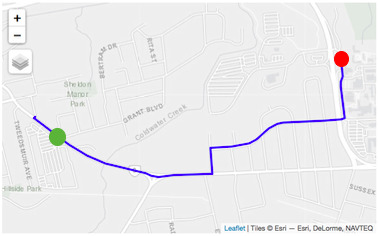
\includegraphics[width=0.65\linewidth]{Route 1A} 

}

\caption{Map of route 1A.}\label{fig:figure-2}
\end{figure}

Most participants reported being familiar with this route; they had
previously cycled at least part of the route or in this general area.
The majority of participants disliked the segments with a four-lane
arterial road that lacked infrastructure, and more than half stated that
they would not cycle this part of the route. Factors that made them
dislike these segments include the lack of cycling facilities, number of
traffic lanes, the width of the lanes, and the hilliness (see Figures 3
and 4). Most participants expected car traffic to be moving faster on
these segments.

\begin{figure}

{\centering 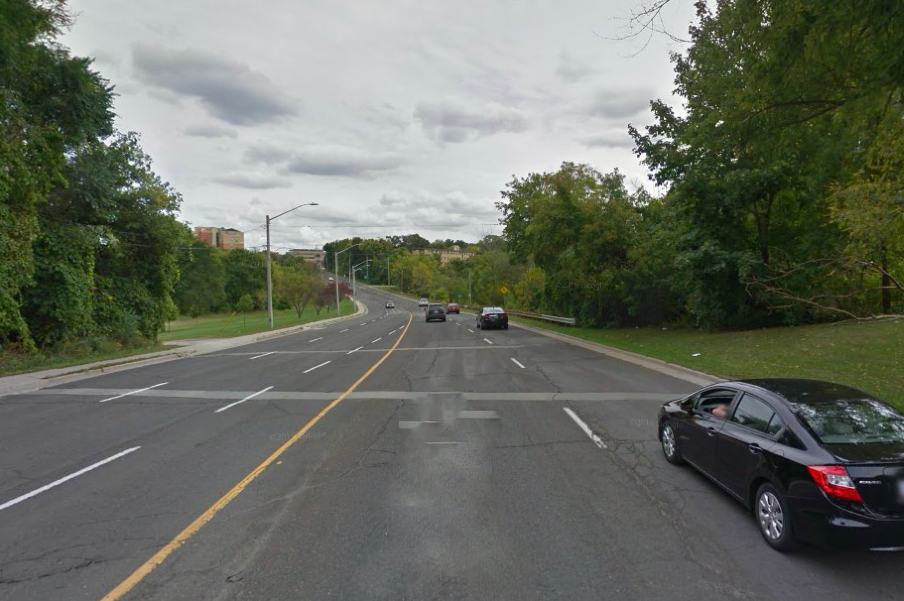
\includegraphics[width=0.65\linewidth]{Figure 3} 

}

\caption{Segment 2 of route 1A depicting two or three lanes in each direction and no cycling facilities on the roadway. Lighting and natural views are present. (Source: Google Street View)}\label{fig:figure-3}
\end{figure}

\begin{figure}

{\centering 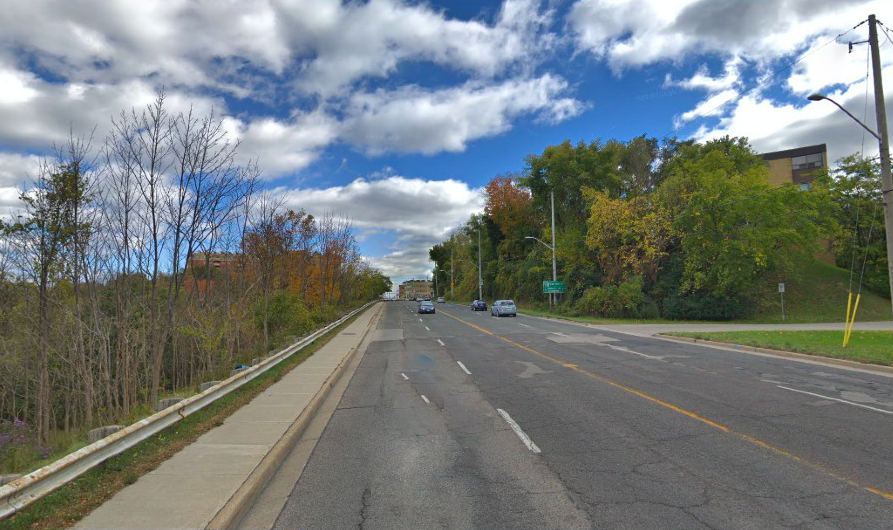
\includegraphics[width=0.65\linewidth]{Figure 4} 

}

\caption{Segment 2 of route 1A depicting the uphill section on a 2 lane arterial road with no on-street cycling infrastructure. (Source: Google Street View)}\label{fig:figure-4}
\end{figure}

A few participants who were familiar with the area reported that they
would have cycled the Hamilton-Brantford Rail Trail instead, an
off-street multi-use trail parallel to the arterial road. Some cyclists
noted that there was no sidewalk or shoulder on the right side of the
roadway where they would be cycling, with some describing that it would
make them feel ``\emph{uncomfortable}'' or ``\emph{anxious}'' without
that space. In general, the arterial road without infrastructure was
perceived to be too busy and not designed for cycling. The left turn at
an unsignalized intersection was also noted as difficult by a few
participants (see Figure 5).

\begin{figure}

{\centering 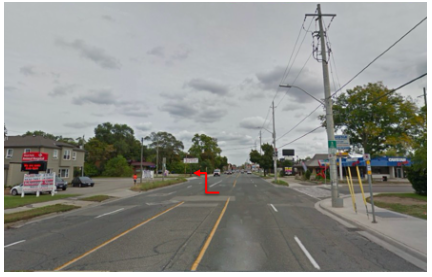
\includegraphics[width=0.65\linewidth]{Figure 5} 

}

\caption{Segment 4 of route 1A depicting the urban design of the street when making a left turn to follow the City's signed bicycle route. (Source: Google Street View)}\label{fig:figure-5}
\end{figure}

However, the route was generally perceived positively once it entered a
residential area. The majority of participants reported liking or had
positive comments of the segments that had an on-street marked bicycle
lane (see Figure 6). Most participants also liked these segments because
they were perceived to be ``\emph{residential}'' or ``\emph{quiet}'',
and not as busy in terms of car volume. Some participants reported
liking the green space and nature along the on-street marked bicycle
lane. In addition, half of the participants stated that they liked the
pedestrian-activated traffic signal because it enabled them to cross the
arterial road promptly and safely (see Figure 7).

\begin{figure}

{\centering 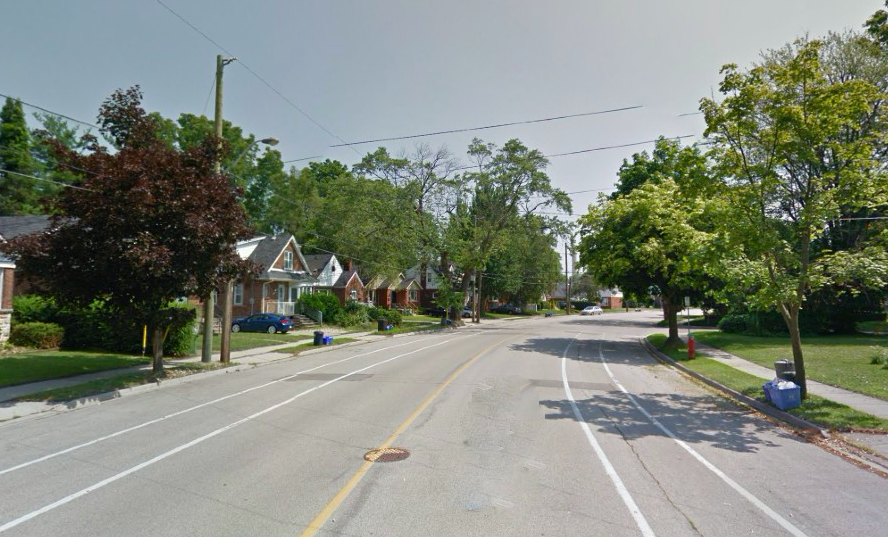
\includegraphics[width=0.65\linewidth]{Figure 6} 

}

\caption{Segment 9 of route 1A depicting the on-street marked bicycle lane in a residential neighbourhood. (Source: Google Street View)}\label{fig:figure-6}
\end{figure}

\begin{figure}

{\centering 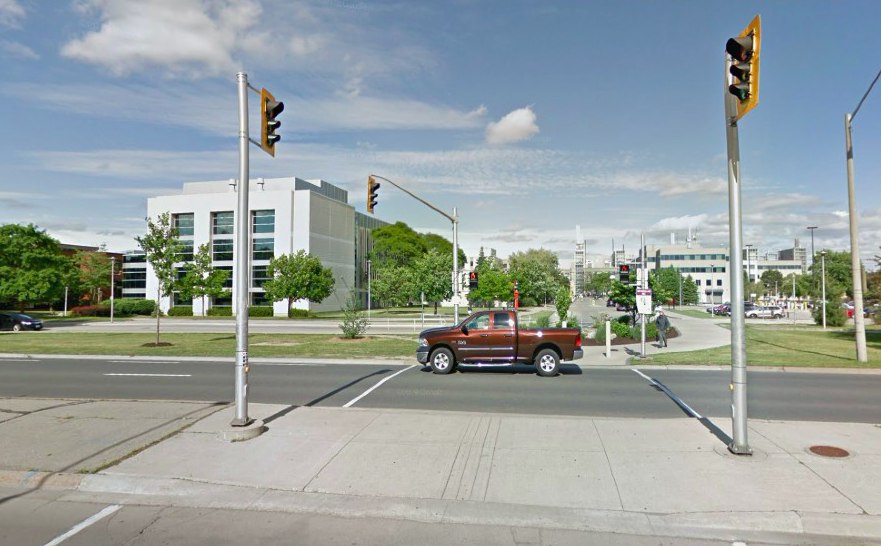
\includegraphics[width=0.65\linewidth]{Figure 7} 

}

\caption{Segment 13 of Route 1A depicting a pedestrian-activated signal to cross a an arterial road. (Source: Google Street View)}\label{fig:figure-7}
\end{figure}

\hypertarget{route-1b}{%
\paragraph{Route 1B}\label{route-1b}}

\begin{figure}

{\centering 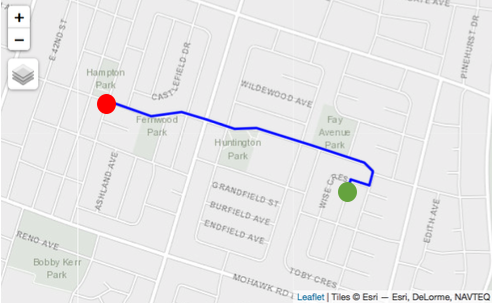
\includegraphics[width=0.65\linewidth]{Route 1B} 

}

\caption{Map of route 1B.}\label{fig:figure-8}
\end{figure}

While none of the participants were familiar with this route, this route
received overall positive comments. Cyclists primarily liked the route
because it was perceived to have low traffic, fewer cars, and was quiet
or residential. Some words used to describe the route include
``\emph{nice}'', ``\emph{lots of trees}'', and ``\emph{not busy}'' (see
Figure 9). The lack of infrastructure was noted by some participants but
only two reported that they disliked this aspect of the route. Only one
participant noticed that it was a signed route, but participants
reported that they would generally feel comfortable cycling this route.
A few participants commented on the good quality of the pavement.
Although the route was perceived to be low traffic and residential, some
cyclists would still have preferred if the route had a dedicated cycling
facility. Four participants noticed or liked the 40 kilometres/hour
speed limit on the route.

\begin{figure}

{\centering 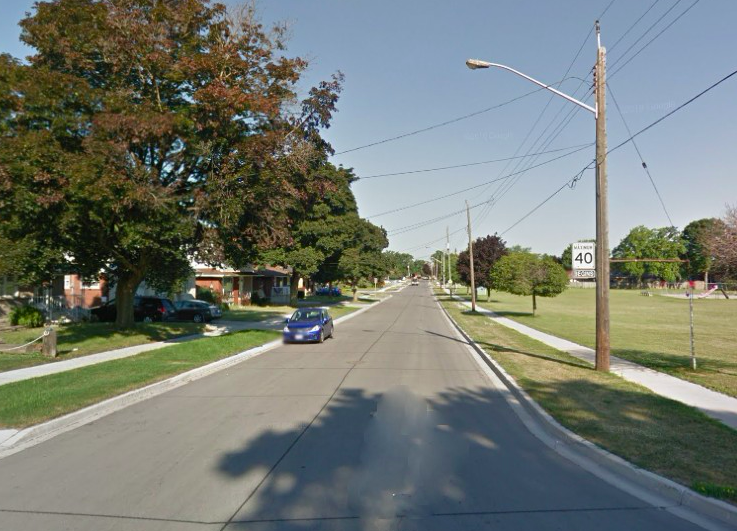
\includegraphics[width=0.65\linewidth]{Figure 9} 

}

\caption{Segment 4 of route 1B depicting the streetscape on a signed route in a residential area. (Source: Google Street View)}\label{fig:figure-9}
\end{figure}

\hypertarget{package-2}{%
\subsubsection{Package 2}\label{package-2}}

\hypertarget{route-2a}{%
\paragraph[Route 2A]{\texorpdfstring{Route 2A\footnote{This route was
  slightly adjusted for the audit. CycleStreets inferred that cyclists
  would cross midblock at an unsignalized intersection towards the end
  of the route. Cyclists have been found to be sensitive to
  intersections Broach et al. (2012). Therefore, the audited route was
  adjusted to a parallel street one block east that would enable a
  cyclist to cross at a signalized intersection.}}{Route 2A}}\label{route-2a}}

\begin{figure}

{\centering 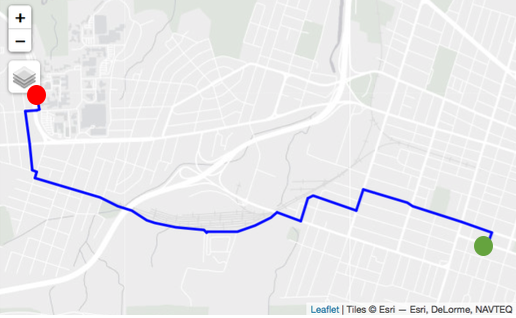
\includegraphics[width=0.65\linewidth]{Route 2A} 

}

\caption{Map of route 2A.}\label{fig:figure-10}
\end{figure}

Participants were familiar with this route and had previously cycled the
entire route or parts of it. Cyclists reported liking the
infrastructure, particularly the on-street marked bicycle and the
Hamilton-Brantford Rail Trail, which is an off-street multi-use path
(see Figure 11 and Figure 12). The Rail Trail was perceived to be ideal
for cycling: one participant called it a ``\emph{superhighway for
bicycles}'', another described it as a fundamental ``\emph{arterial
route}'' for cyclists in Hamilton. Most participants also liked that
many sections of the route that did not have dedicated infrastructure
were on residential streets. Several cyclists liked or noticed that the
route connected them to or passed by key destinations.

\begin{figure}

{\centering 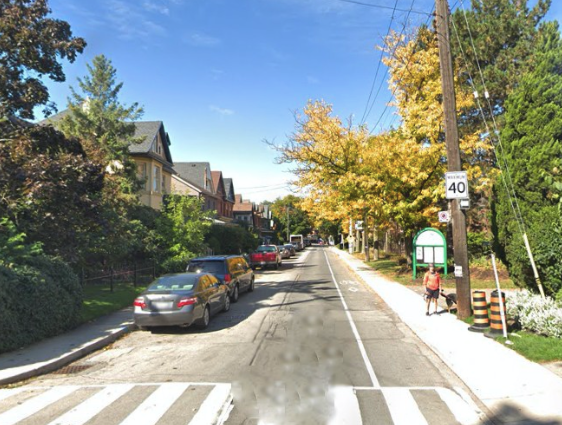
\includegraphics[width=0.65\linewidth]{Figure 11} 

}

\caption{Segment 5 on route 2A depicting an on-street marked bicycle lane on a one-way street with one lane going westward. (Source: Google Street View)}\label{fig:figure-11}
\end{figure}

\begin{figure}

{\centering 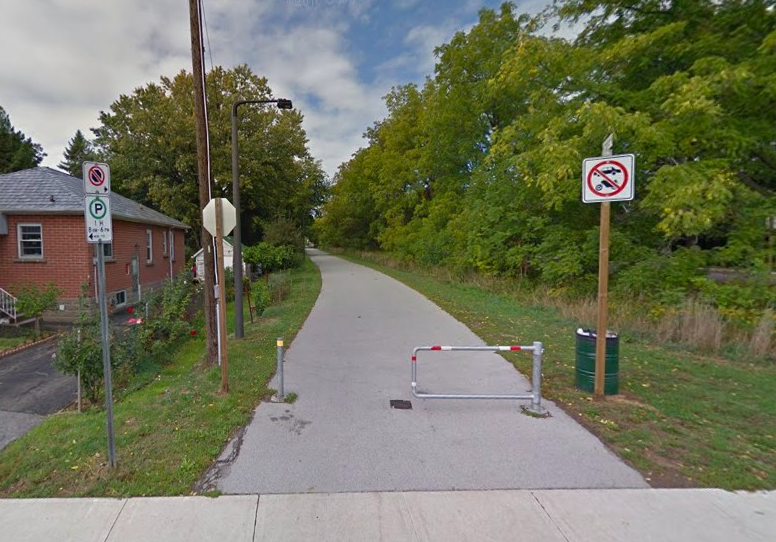
\includegraphics[width=0.65\linewidth]{Figure 12} 

}

\caption{Segment 18 of route 2A depicting the off-street multi-use path called the Hamilton Brantford Rail Trail. (Source: Google Street View)}\label{fig:figure-12}
\end{figure}

There were four areas or features along the route that participants
disliked or that were more poorly perceived. First, several participants
disliked or expressed concern about turning left at an intersection
without a signal after the bike lane ends. Cyclists who disliked this
feature reported often waiting a while to turn left, that it was
challenging for them that motorists did not always anticipate their need
to transition lanes like other road users, or that they were not given
enough space (see Figure 13).

\begin{figure}

{\centering 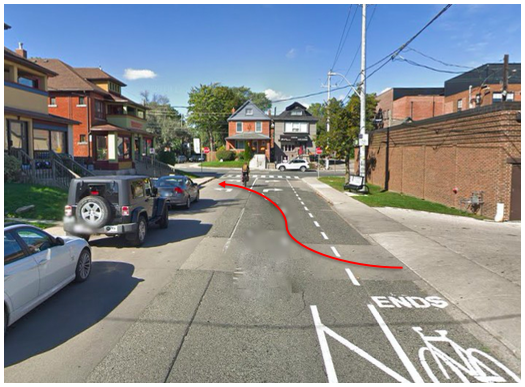
\includegraphics[width=0.65\linewidth]{Figure 13} 

}

\caption{Segment 8 of route 2A depicting the buffered bicycle lane ending and the transition that a cyclist would have to make to get into the left-turn lane. (Source: Google Street View)}\label{fig:figure-13}
\end{figure}

Second, the short stretch along an arterial road with two traffic lanes
in each direction and no dedicated cycling infrastructure (see Figure
14) was strongly disliked by most participants. Others had mixed
perceptions or experiences or reported being fine cycling on a short
stretch of this road. Those who strongly disliked the arterial road
reported avoiding this street as much as possible or preferred to cycle
on the sidewalk instead. For example, the arterial road was perceived to
be a ``\emph{speedway}'' and an area that had ``\emph{a lot of car
entitlement}''. Next, the left turn at a signalized intersection from an
arterial road to a street with sharrows was disliked or concerning for
some participants (see Figure 15). Many participants noted that they
used an alternate route to get to the Rail Trail to avoid this arterial
road and intersection entirely.

\begin{figure}

{\centering 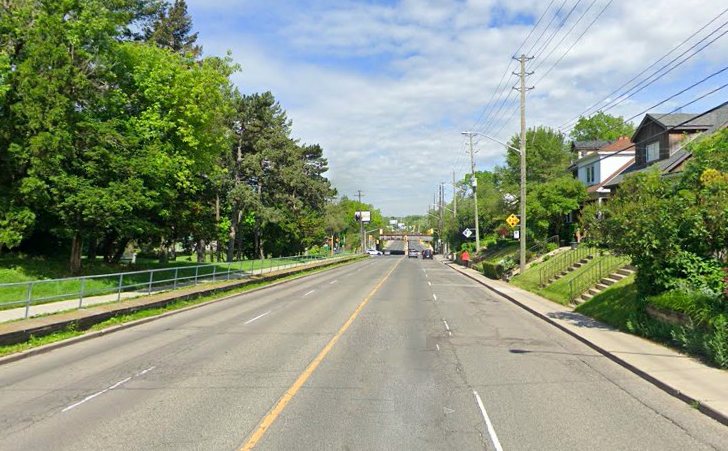
\includegraphics[width=0.65\linewidth]{Figure 14} 

}

\caption{Segment 14 of route 2A depicting an arterial road without on-street cycling infrastructure. (Source: Google Street View)}\label{fig:figure-14}
\end{figure}

\begin{figure}

{\centering 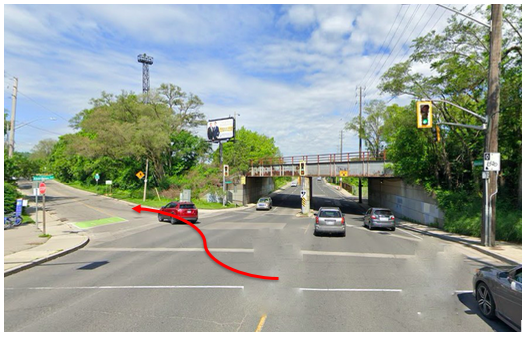
\includegraphics[width=0.65\linewidth]{Figure 14a} 

}

\caption{Segment 14 of route 2A depicting a signalized intersection where a cyclist would turn left on to a street with sharrows to travel to the Hamilton-Brantford Rail Trail. (Source: Google Street View)}\label{fig:figure-15}
\end{figure}

Finally, most cyclists stated that they disliked an intersection at the
end of the route that would require them to transition from a
residential to arterial road (see Figure 16). The area was viewed as
very busy or ``\emph{not fluid}'' by some participants because there was
an off-street multi-use path parallel to the road on the left side of
the roadway that could not be accessed swiftly from the right side.
However, several participants reported that they would have taken an
alternate route to access the university campus from another entrance.

\begin{figure}

{\centering 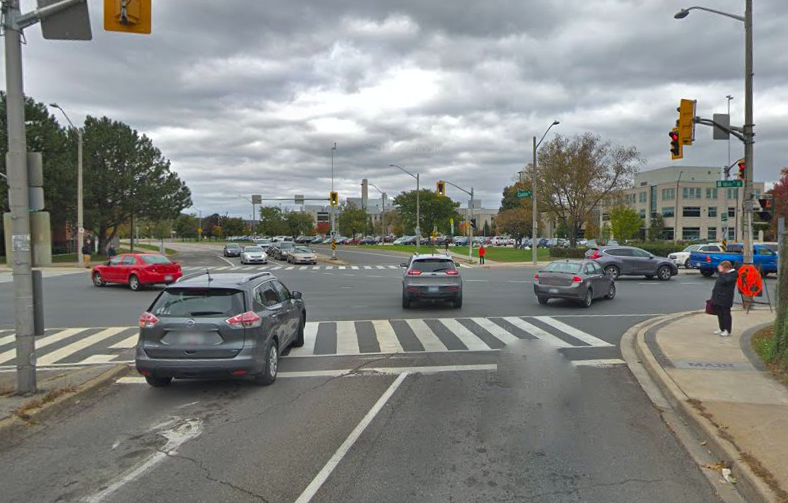
\includegraphics[width=0.65\linewidth]{Figure 15} 

}

\caption{Segment 29 of route 2A depicting the intersection of a residential road and two arterial roads. (Source: Google Street View)}\label{fig:figure-16}
\end{figure}

\hypertarget{route-2b}{%
\paragraph{Route 2B}\label{route-2b}}

\begin{figure}

{\centering 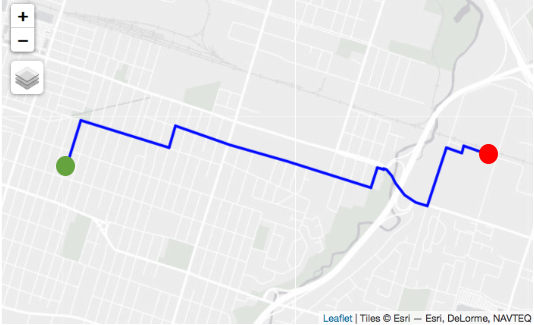
\includegraphics[width=0.65\linewidth]{Route 2B} 

}

\caption{Map of route 2B.}\label{fig:figure-17}
\end{figure}

Some cyclists reported that they were familiar with this route or that
they had previously cycled part of the route. The participants commented
that there was a mix of features of the route that they liked and
disliked. The segments along the route that were perceived to be
``\emph{quiet}'' or ``\emph{residential}'' were liked by most
participants because car volume and speed were perceived to be lower
(see Figure 18). The protected off-street multi-use trail over the
highway was another feature that most participants liked or that
elicited positive comments (see Figure 19). In general, the segments
that were perceived to not be busy with traffic were liked or
participants reported feeling comfortable cycling there, but the
segments where car volume or speed were perceived to be higher were
disliked.

\begin{figure}

{\centering 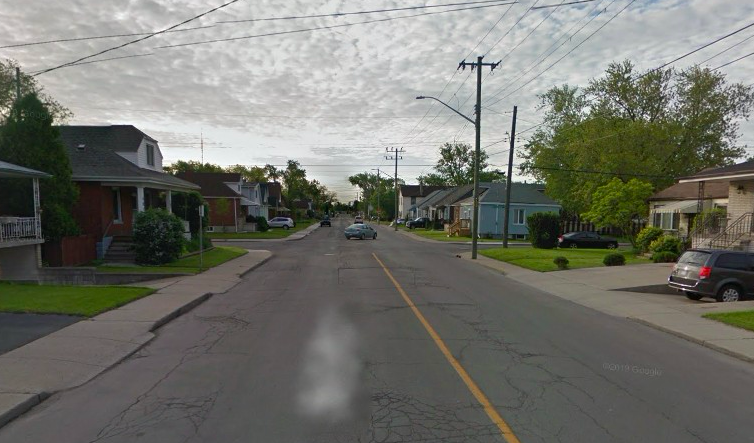
\includegraphics[width=0.65\linewidth]{Figure 17} 

}

\caption{Segment 11 of route 2B depicting a residential area. (Source: Google Street View)}\label{fig:figure-18}
\end{figure}

\begin{figure}

{\centering 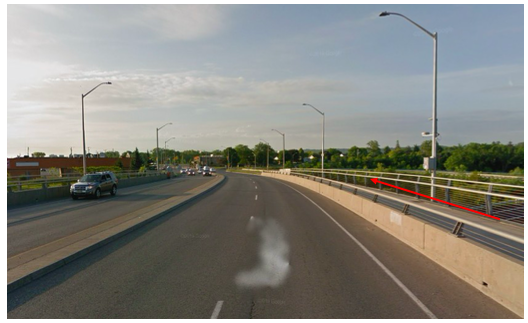
\includegraphics[width=0.65\linewidth]{Figure 18} 

}

\caption{Segment 30 of route 2B depicting the protected multi-use trail on the right side of the roadway on an arterial road over the Red Hill Valley Parkway. (Source: Google Street View)}\label{fig:figure-19}
\end{figure}

Some cyclists had mixed perceptions about the width of some of the
segments (see Figure 20 and Figure 21). A few participants commented
that at times there appeared to be enough space for motorists to safely
pass cyclists, while others perceived the wide streets to potentially
invite speeding. Anticipated car volume and the presence of on-street
parking along these segments seemed to influence perceptions about the
width of the street and comfortability. Cyclists preferred to have space
for a motorist to safely pass. Most participants noticed or disliked the
poor condition of the road along parts of the route. Finally,
participants reported that they disliked the end of the multi-use trail
or having to cycle on an arterial road and cross four lanes to make a
left turn (see Figure 22).

\begin{figure}

{\centering 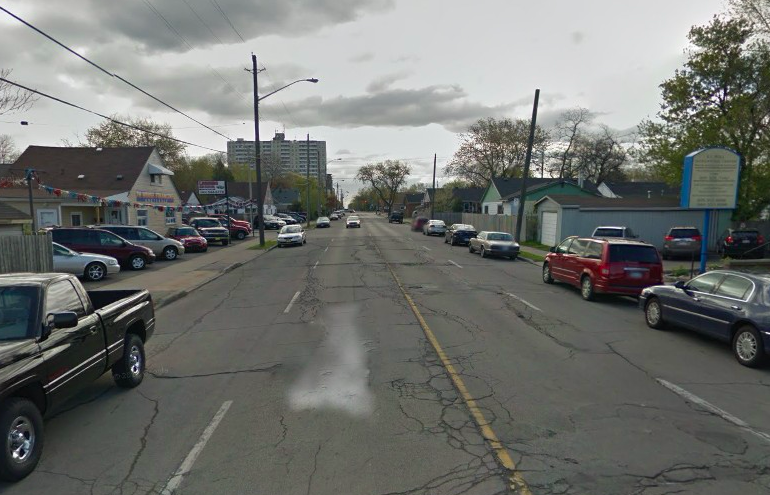
\includegraphics[width=0.65\linewidth]{Figure 19} 

}

\caption{Segment 14 on route 2B depicting a two-lane arterial road with on-street parking. (Source: Google Street View)}\label{fig:figure-20}
\end{figure}
\begin{figure}

{\centering 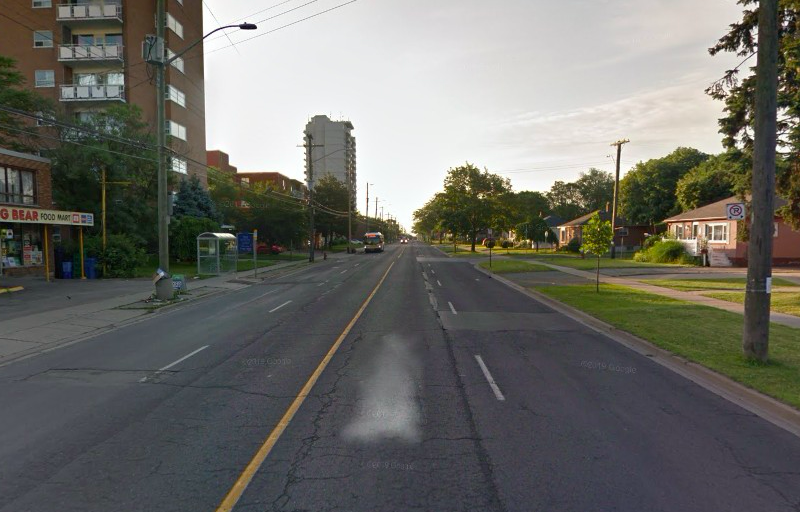
\includegraphics[width=0.65\linewidth]{Figure 20} 

}

\caption{Segment 20 on route 2B depicting a two-lane arterial road with no on-street parking and a wide grassy verge on the right side of the roadway. (Source: Google Street View)}\label{fig:figure-21}
\end{figure}

\begin{figure}

{\centering 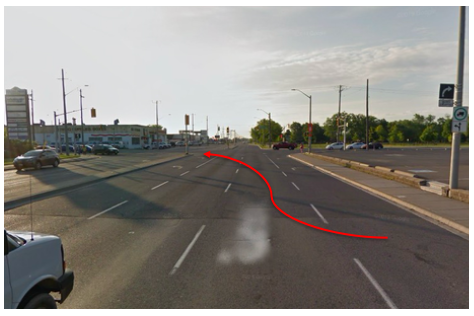
\includegraphics[width=0.65\linewidth]{Figure 21} 

}

\caption{Segment 31 of route 2B depicting a lane change from the far right side of the roadway to the left-turn lane on a four-lane arterial road. (Source: Google Street View)}\label{fig:figure-22}
\end{figure}

\hypertarget{package-3-1}{%
\subsubsection{Package 3}\label{package-3-1}}

\hypertarget{route-3a}{%
\paragraph[Route 3A]{\texorpdfstring{Route 3A\footnote{This route was
  slightly adjusted for the audit. The starting point was midblock on a
  residential street. The audit started instead at the nearest
  intersection along the route.}}{Route 3A}}\label{route-3a}}

\begin{figure}

{\centering 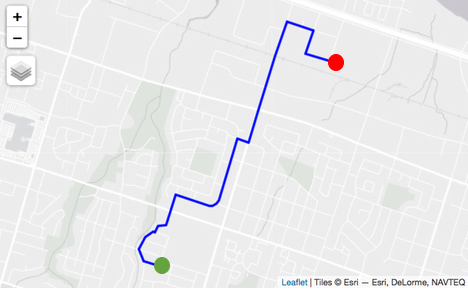
\includegraphics[width=0.65\linewidth]{Route 3A} 

}

\caption{Map of route 3A.}\label{fig:figure-23}
\end{figure}

None of the participants had cycled in this area or were familiar with
this route. The opposite to Route \emph{1A}, participants liked the
first half of the route and generally disliked features of the second
half. The beginning of the route was in a residential area; most
cyclists reported that they liked the quiet streets and good road
condition (See Figure 24). The lower speed limit of 40 kilometres/hour
was noticed by several participants and some commented that they like
travelling on streets with this speed limit. Once the route left the
residential area about mid-way, most participants disliked turning to or
cycling on a two-lane arterial road without infrastructure. The arterial
road leading towards the industrial was perceived by some cyclists to be
designed for cars (see Figure 25 and Figure 26). One participant
described this as, ``\emph{you're just out on a bike in the middle of
the highway}''. The route ended in an industrial area which received
mixed perceptions; some cyclists commented that traffic volume did not
appear to be too heavy in the photos while many others reported feeling
less comfortable cycling in an area where they could expect a lot of
trucks.

\begin{figure}

{\centering 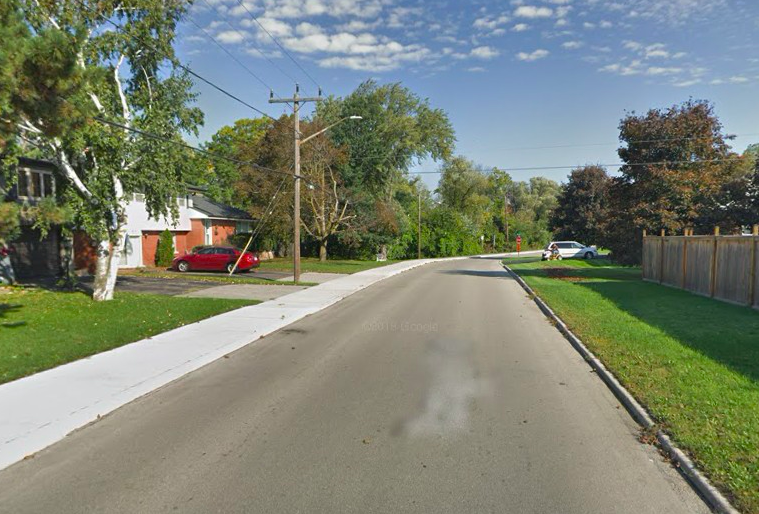
\includegraphics[width=0.65\linewidth]{Figure 23} 

}

\caption{Segment 2 of route 3A depicting a residential street. (Source: Google Street View)}\label{fig:figure-24}
\end{figure}

\begin{figure}

{\centering 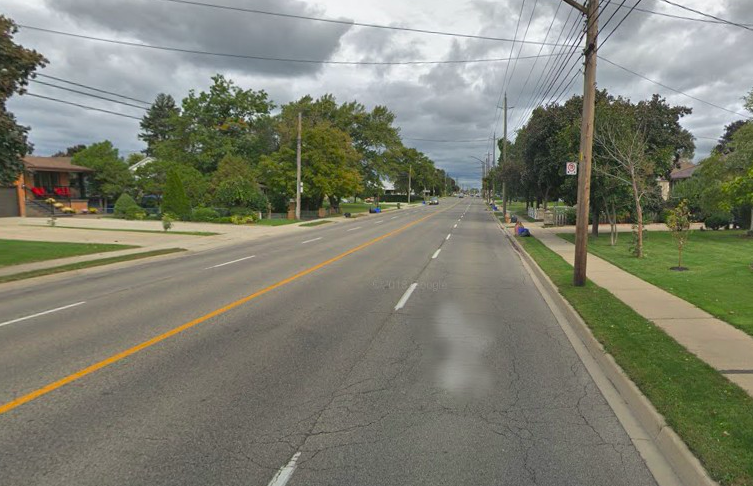
\includegraphics[width=0.65\linewidth]{Figure 24} 

}

\caption{Segment 13 of route 3A depicting a two-lane arterial road without cycling facilities in a residential area. (Source: Google Street View)}\label{fig:figure-25}
\end{figure}

\begin{figure}

{\centering 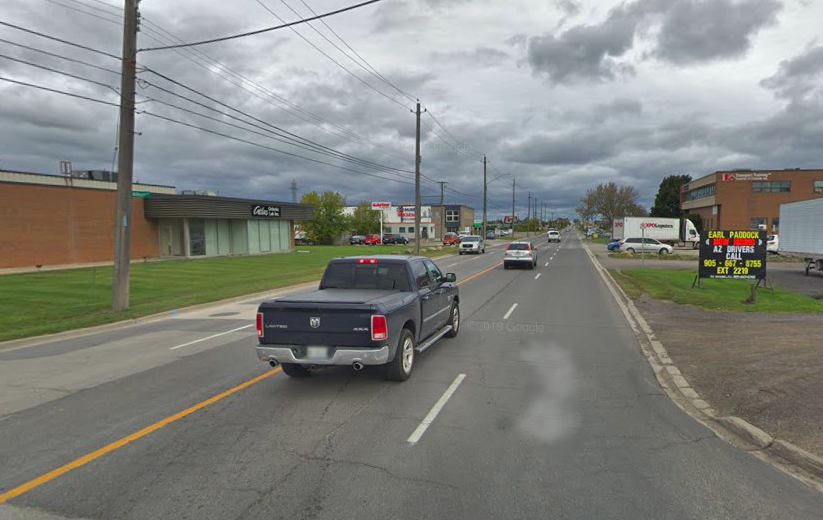
\includegraphics[width=0.65\linewidth]{Figure 25} 

}

\caption{Segment 15 of route 3A depicting a two-lane arterial road without cycling facilities or a sidewalk leading to a more industrial area. (Source: Google Street View)}\label{fig:figure-26}
\end{figure}

\hypertarget{route-3b}{%
\paragraph[Route 3B]{\texorpdfstring{Route 3B\footnote{This route was
  slightly adjusted for the audit. Rather than starting midblock on an
  uphill access to the escarpment, which would be an unlikely origin,
  the audit started two blocks south. Recall that the origin of each
  inferred route is the centroid of the traffic analysis zone, so this
  is not the true origin of this cycling flow.}}{Route 3B}}\label{route-3b}}

\begin{figure}

{\centering 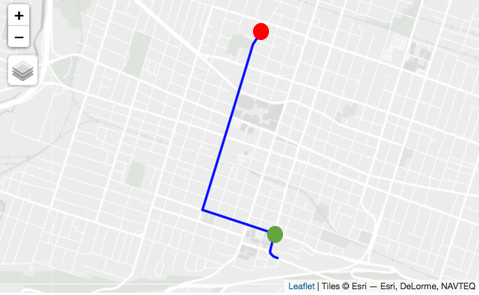
\includegraphics[width=0.65\linewidth]{Route 3B} 

}

\caption{Map of route 3B.}\label{fig:figure-27}
\end{figure}

This route was familiar to the participants and the majority had cycled
at least part of it. Cyclists liked that the majority of the route had
cycling infrastructure (see Figure 28 and 29). The first few segments at
the beginning of the route were perceived to be busy in terms of traffic
by several participants, but many noted that people drive slower near
the hospital.

\begin{figure}

{\centering 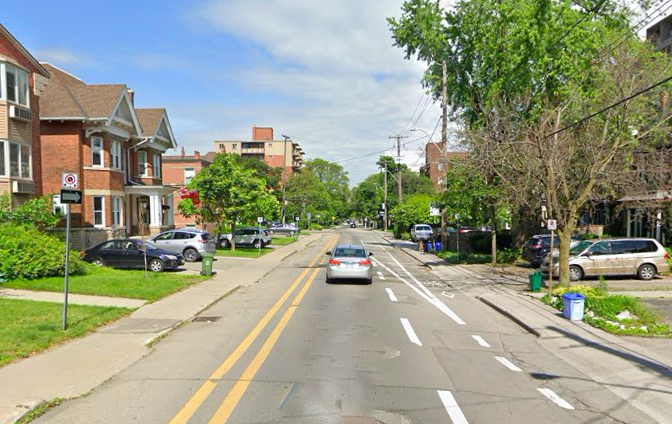
\includegraphics[width=0.65\linewidth]{Figure 27} 

}

\caption{Segment 4 on route 3B with a buffered on-street bicycle lane on a one-way street. (Source: Google Street View)}\label{fig:figure-28}
\end{figure}

The two-way cycle track (see Figure 29) was generally perceived well and
elicited a lot of comments from participants, likely because they
reported using it. However, participants expressed a mix of appreciation
and frustration about this ``\emph{major cycling infrastructure}''.
Several participants reported that they had witnessed people drive or
park in the lanes, as well as drift into them to avoid passing closely
to the parked cars in the outer right lane. Many participants expressed
a desire to have enhanced protection along these facilities. Three
participants, one travelling with a young child, reporting being hit by
a motorist who was turning left across the cycle track. Others reported
being vigilant when using this infrastructure because it is a two-way
facility on a one-way street. Despite it being a relatively new and
important North-South route in the city's cycling network, cyclists
described that it needed improvements in particular areas that were
conflict points with other road users.

\begin{figure}

{\centering 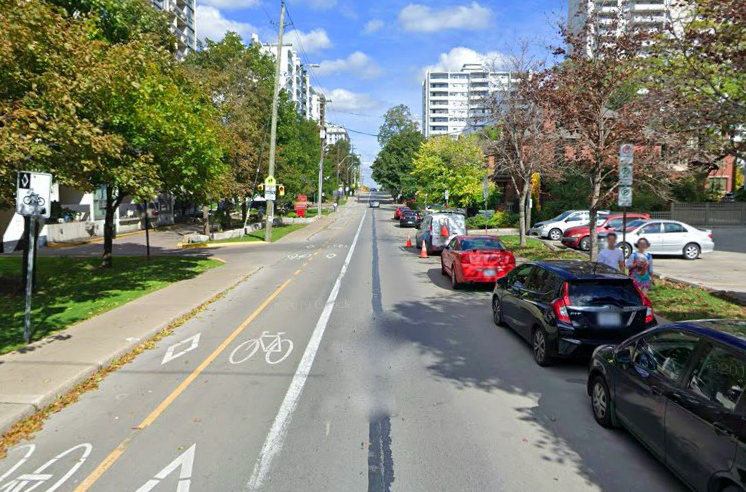
\includegraphics[width=0.65\linewidth]{Figure 28} 

}

\caption{Segment 8 on route 3B depicting a two-way cycle track on a one-way arterial road. (Source: Google Street View)}\label{fig:figure-29}
\end{figure}

There were also mixed comments about a few intersections along the route
that had bike boxes. Most cyclists reported that this infrastructure
could be confusing, both for them and for motorists, and that sometimes
motorists park in them if the light is red (see Figure 30). However,
others reported that they liked the bike boxes and find them useful for
transition points. The route was also perceived to be disconnected or
disjointed by some participants; these comments were in reference to the
different or inconsistent types of infrastructure along the route and
because the infrastructure ends or is missing at certain spots.

\begin{figure}

{\centering 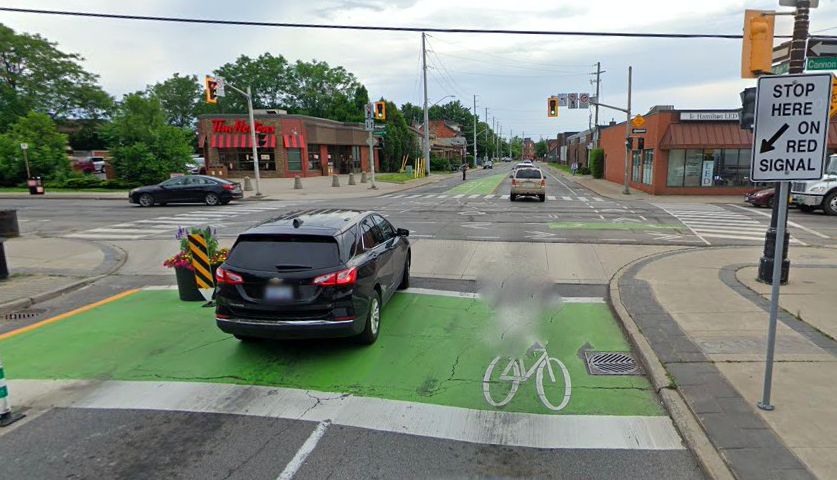
\includegraphics[width=0.65\linewidth]{Figure 29} 

}

\caption{Segment 20 of route 3B depicting the bike box at the intersection of two cycling facilities. After the intersection, the two-way cycle track on the left side of the roadway splits to on-street bicycle lanes on both sides of the road. (Source: Google Street View)}\label{fig:figure-30}
\end{figure}

\hypertarget{preferred-routes}{%
\subsection{Preferred Routes}\label{preferred-routes}}

After reviewing each of the three packages of photos, participants were
asked to select which of the two routes in each package they preferred.
All participants consistently selected the same routes: \emph{1B} was
preferred over \emph{1A}, \emph{2A} over \emph{2B}, and \emph{3B} over
\emph{3A}. In the first package, cyclists preferred route \emph{1B}
because they disliked the first three segments of \emph{1A}. Cycling on
route \emph{1B} on residential streets was preferred over negotiating
shared space on a busy four-lane arterial road even though there were
dedicated cycling facilities later in the route. It is worth noting that
a few participants commented that they most preferred the second half of
\emph{1A} because it had an on-street marked bicycle lane, but that
\emph{1B} was a better route overall. In the second package,
participants preferred \emph{2A} because it had cycling infrastructure
throughout compared to \emph{2B} which had a signed route only for part
of it. \emph{2A} was also familiar to most participants. Finally,
\emph{3B} was preferred for similar reasons that \emph{2A} was
preferred; there were on-street cycling facilities for most of the route
and it was familiar to most participants.

\hypertarget{sec:discussion}{%
\section{Discussion}\label{sec:discussion}}

The environmental audits revealed that each of the routes had a mix of
attributes that support or hinder cycling. This can be expected in a
city with a cycling network under development. The audits helped to
explain why certain trip flows were over- or under-estimated by the
model {[}paper submitted to \emph{Transportation}{]}. All inferred
routes included residential streets with lower volumes of cars or
cycling infrastructure. With respect to the routes that were
under-estimated (i.e., \emph{1B}, \emph{2B}, \emph{3A}, and \emph{3B}),
there were many features that might influence cycling. For instance, two
of the four (i.e., \emph{2B} and \emph{3B}) had some type of separated
cycling facility. Three of the four routes (i.e., \emph{1B}, \emph{2B},
and \emph{3A}) included residential streets. Based on the routes
audited, we observed that the \emph{CycleStreets} algorithm makes
sensible recommendations that a knowledgeable cyclist could take.
Indeed, three of the six routes (\emph{1A}, \emph{2A}, and \emph{3B})
were familiar to or had been previously cycled by many participants.
This suggests that the inferred routes do match where cyclists actually
travel in Hamilton.

Participants preferred routes that visibly accommodate cycling, and
their route and infrastructure preferences align with previous
literature. They preferred cycling facilities and streets with lower
levels of traffic, which has been found in many other studies
(\emph{inter alia}, see Buehler and Dill, 2016; Clark et al., 2019;
Mertens et al., 2017; Winters et al., 2011). Participants were also
sensitive to traveling through intersections (Broach et al., 2012) and
many enjoyed routes that had natural features (Marquart et al., 2020;
Winters et al., 2011). Perceived car volume was another factor that
participants frequently commented on as they reviewed photos, likely
because cyclists are known to be sensitive to busy traffic (Segadilha
and Sanches, 2014) and are motivated to cycle if there are routes away
from cars (Winters et al., 2011). Cyclists in Hamilton describe similar
experiences to those who cycle in Waterloo, Ontario (Mayers and Glover,
2020), which suggests that a pattern of exclusion may currently exist in
mid-sized cities as they grapple with a tension between transport
culture and new interventions. Finally, participants also considered a
range of factors beyond infrastructure to determine whether a street or
route sufficiently meets their needs and preferences, which is useful
information for policy-makers and transport planners. Many participants
reported that they like to cycle on roads with smooth or good
conditions, which has previously been reported in the literature
(Stinson and Bhat, 2003). Some cyclists preferred to have lateral space
to their right, like a sidewalk or some other ``\emph{escape zone}'', in
the event that they needed to quickly move out of the way. These
attributes may be overlooked by transport planners but should be
considered when planning cycling networks and routes.

The temporal aspect of our photo elicitation approach also revealed that
there is a threshold of unpleasantness that cyclists are willing to
tolerate along a route. In the case of route \emph{1A}, the segments
along the arterial road without infrastructure were such strong
deterrents that cyclists preferred the other unfamiliar residential
route. Although \emph{1A} was inferred and not one that participants
reported using, someone who is new to cycling but unfamiliar with other
routes could likely consider this to be the most direct route. The photo
activity underscored that the fragmented nature of the cycling network
in a developing cycling city can create barriers for accessing bikeable
streets. This reinforces the importance of connected facilities in
encouraging cycling (Buehler and Dill, 2016; Handy, 2020; Yang et al.,
2019) and that navigating mixed traffic in cities where there is less
infrastructure is perceived to be less safe (Chataway et al., 2014).
More importantly, these streets are not separate from the rest of the
transport system and the ability to reach this infrastructure matters.
If getting to on-street cycling facilities is perceived to be
challenging or too dangerous, then regular and even potential cyclists
may be unwilling to use existing infrastructure or avoid routes that
incorporate these streets altogether.

\hypertarget{policy-implications}{%
\subsection{Policy Implications}\label{policy-implications}}

There are three important implications of this study for developing
cycling cities: i) the perceptions of cyclists should be regularly
explored and incorporated in route design; ii) the timing of
incorporating cyclists' feedback is important for ensuring that
infrastructure is functional and adapted as it grows; and iii) using
photo elicitation is an innovative and practical approach for planning
practice.

Although our approach differed from other studies where participants
took photos themselves (Bornioli et al., 2018; Guell and Ogilvie, 2015;
Ward et al., 2015), the photo activity was illuminating because it
helped participants recall their experiences and revealed rich insights
about cycling behaviours and perceptions. This evidence could not have
been derived from a travel survey or cycle routing algorithm. This is
one of the benefits of using photos to elicit dialogue because they
``evoke deeper elements of human consciousness than do words'' (Harper,
2002). Therefore, it is recommended that developing cycling cities
routinely examine cycling perceptions through qualitative data like
photo elicitation to centre the experience of cycling in the design of
infrastructure and routes. This data can also be useful for mobile
applications based on crowdsourced data or digital platforms that
incorporate cyclists' informal routes to inform future cycling route and
new locations for infrastructure (see Cellina et al., 2020; Meireles and
Ribeiro, 2020). Users can describe how particular routes or types of
infrastructure are actually experienced and travelled, both to
communicate preferred routes to other cyclists and to highlight
necessary improvements to planners. The use of photos can extend current
planning practices beyond simple identification of problem areas by
describing how cyclists navigate these spaces.

Furthermore, inviting cyclists to have a more regular participatory role
in route design and planning as the cycling network develops is an
important practice. Failing to understand and integrate cyclists'
perceptions and preferences in planning early on in a city's cycling
network development can negatively impact efforts to increase cycling;
resources could be spent on facilities that are fundamentally
unappealing to cyclists or other barriers can be ignored. Taking
advantage of cyclists' expertise in developing cycling cities can help
to overcome the barrier of a lack of safe cycling routes, a barrier
identified in another ``low cycling maturity'' city by Félix et
al.~(2019). Marquart et al.'s (2020) study highlights that planners
``are determining the characteristics of routes in urban areas'', which
supports our recommendation that more opportunities be created for
cyclists to share feedback. Without such opportunities, tools can be
developed that only reflect the designers' perceptions and that fail to
account for the needs of other cyclists like women (Xie and Spinney,
2018). Participants' comments about the bike boxes, a relatively new
cycling intervention in Hamilton, is one example of how the use of
photos and detailed feedback can be informative for transport planners.
Likewise, new or potential cyclists also have specific preferences and
their perceptions should be explored through similar approaches. In
addition to our methods, other mapping techniques (see Manton et al.,
2016; Marquart et al., 2020), ride-along activities (see van Duppen and
Spierings, 2013), and frequent audits before and after next
infrastructure is built may be further informative for understanding how
cyclists navigate developing cycling cities.

Finally, transport planners in developing cycling cities, like Hamilton,
should make every effort to focus beyond infrastructure and seek to
better integrate these individual links within a transport system that
is designed with pro-cycling policies in mind. Studies have provided
evidence that cities that are most successful in increasing their
cycling trips and levels have implemented a suite of interventions to
change behaviour and the built environment (Pucher et al., 2011, 2010).
Our findings support the recommendation that the City of Hamilton
explore and implement bolder policies to encourage modal shifts. There
is strong incentive for prioritizing cycling more: 35\% of all current
trips in Hamilton could be cycled (Mitra et al., 2016) and more people
could benefit from increased physical activity.

\hypertarget{sec:limitations}{%
\section{Study Limitations}\label{sec:limitations}}

There are some instances where the \emph{CycleStreets} algorithm failed
to include some of the city's off-street cycle infrastructure or signed
routes. Some participants noted these situations and described alternate
detours that are more locally known. This highlights that a routing
algorithm may not reflect the extent or range of behaviours of cyclists.
However, many routes were familiar to participants so we find that the
algorithm makes sensible recommendations. Although the photos of the
routes were taken from Google Street View and may not reflect prime
cycling times and likely traffic volumes expected at those times, there
were no errors or differences pointed out by participants along routes
familiar to them.

Furthermore, several cyclists noted that the routes they preferred were
familiar to them, which suggests that familiarity played a role in their
decision. This makes sense because it affords them more intimate
knowledge of the route. Therefore, our findings could have been
different if the participants were familiar with all of the routes or if
they were familiar with none. However, their familiarity offered
insightful information about how these road spaces are actually
experienced which is useful for transport planners in Hamilton. Our
findings would also likely have been different if the participants were
new or occasional cyclists. Less experienced cyclists are likely to have
even stronger preferences for protected infrastructure and be more
averse to mixing with traffic (Winters et al., 2011). The findings may
not match the preferences or experiences of other cyclists such as older
adults, women who are more conscious of traffic risks, children, or
marginalized groups. These individuals have unique needs with respect to
separation from traffic and perceptions of the built environment, as
well as different trip patterns (\emph{inter alia} see Aldred, 2015;
Black and Street, 2014; Emond et al., 2009).

Finally, some photos taken from Google Street View were darker or
cloudier than others. This was noticed by some participants, suggesting
that it may have subconsciously influenced participants' perceptions.
However, there was similarity in participants' stated preferences and
all selected the same preferred routes. This suggests the weather
depicted in the photos likely had less of an influence on individual
perceptions and preferences, and that attributes of the routes and
familiarity were more important.

\hypertarget{sec:conclusion}{%
\section{Conclusion}\label{sec:conclusion}}

Through environmental audits and a photo activity in semi-structured
interviews we demonstrated that cycling routes in Hamilton have a mix of
attributes that support and hinder cycling. The interviews with regular
cyclists revealed that they prefer routes that have dedicated cycling
infrastructure or streets with low volumes of traffic, and that existing
infrastructure needs to be adapted to better align with cyclists' needs
and preferences. As a developing cycling city with 46\% of the cycling
network completed, the findings from this study will be useful to
policy-makers and transport planners in Hamilton, and other mid-sized
cities with growing cycling levels, to design more bicycle-friendly
streets and facilitate more trips that enable people to be physically
active. Our findings support the recommendation that other developing
cycling cities involve local cyclists to inform infrastructure design
and location and pay attention to a broad range of built environment
factors that influence where people choose to cycle. The use of photos
to explore cyclists' perceptions and experiences is a promising
participatory approach that can be incorporated into planning practice
to complement travel survey data and better centre the cycling
experience in cycle infrastructure and route design.

\hypertarget{sec:acknowledgments}{%
\section{Acknowledgments}\label{sec:acknowledgments}}

The authors wish to express their sincere gratitude to the participants
of the study who shared their time and stories. The authors also wish to
thank the research assistants for their assistance in collecting data
and conducting the environmental audits. In addition, the following
\texttt{R} packages were used in the course of this investigation and
the authors wish to acknowledge their developers: \texttt{cyclestreets}
(Lovelace and Lucas-Smith, 2018), \texttt{dplyr} (Wickham et al., 2021),
\texttt{float} (Schmidt and Chen, 2020), \texttt{forcats} (Wickham,
2020), \texttt{ggplot2} (Wickham et al., 2020), \texttt{ggthemes}
(Arnold, 2019), \texttt{kableExtra} (Zhu, 2020), \texttt{knitr} (Xie,
2021), \texttt{ngram} (Schmidt and Heckendorf, 2017), \texttt{purrr}
(Henry and Wickham, 2020), \texttt{readr} (Wickham and Hester, 2020),
\texttt{rticles} (Allaire et al., 2021), \texttt{sf} (Pebesma, 2021),
\texttt{sp} (Pebesma and Bivand, 2021), and \texttt{spdep} (Bivand,
2020).

\hypertarget{sec:credit}{%
\section{CRediT Statement}\label{sec:credit}}

\textbf{First author}: conceptualization, methodology, investigation,
formal analysis, data curation, writing - original draft, writing -
review \& editing. \textbf{Second author}: conceptualization,
methodology, writing - original draft, writing - review \& editing.
\textbf{Third author}: conceptualization, writing - original draft,
writing - review \& editing. \textbf{Fourth author}: conceptualization,
writing - original draft, writing - review \& editing. \textbf{Fifth
author}: conceptualization, methodology, writing - original draft,
writing - review \& editing, supervision.

\hypertarget{sec:references}{%
\section*{References}\label{sec:references}}
\addcontentsline{toc}{section}{References}

\hypertarget{refs}{}
\leavevmode\hypertarget{ref-adamPlanningCyclingDispersed2020}{}%
Adam, L., Jones, T., te Brömmelstroet, M., 2020. Planning for cycling in
the dispersed city: Establishing a hierarchy of effectiveness of
municipal cycling policies. Transportation 47, 503--527.
doi:\href{https://doi.org/10.1007/s11116-018-9878-3}{10.1007/s11116-018-9878-3}

\leavevmode\hypertarget{ref-aldredAdultsAttitudesChild2015}{}%
Aldred, R., 2015. Adults' attitudes towards child cycling: A study of
the impact of infrastructure. European Journal of Transport and
Infrastructure Research 15.
doi:\href{https://doi.org/10.18757/ejtir.2015.15.2.3064}{10.18757/ejtir.2015.15.2.3064}

\leavevmode\hypertarget{ref-alexanderViewsNeighbourhoodPhotoElicitation2013}{}%
Alexander, V.D., 2013. Views of the Neighbourhood: A Photo-Elicitation
Study of the Built Environment. Sociological Research Online 18, 1--26.
doi:\href{https://doi.org/10.5153/sro.2832}{10.5153/sro.2832}

\leavevmode\hypertarget{ref-R-rticles}{}%
Allaire, J., Xie, Y., R Foundation, Wickham, H., Journal of Statistical
Software, Vaidyanathan, R., Association for Computing Machinery,
Boettiger, C., Elsevier, Broman, K., Mueller, K., Quast, B., Pruim, R.,
Marwick, B., Wickham, C., Keyes, O., Yu, M., Emaasit, D., Onkelinx, T.,
Gasparini, A., Desautels, M.-A., Leutnant, D., MDPI, Taylor and Francis,
Ögreden, O., Hance, D., Nüst, D., Uvesten, P., Campitelli, E.,
Muschelli, J., Hayes, A., Kamvar, Z.N., Ross, N., Cannoodt, R., Luguern,
D., Kaplan, D.M., Kreutzer, S., Wang, S., Hesselberth, J., Dervieux, C.,
2021. Rticles: Article formats for r markdown.

\leavevmode\hypertarget{ref-R-ggthemes}{}%
Arnold, J.B., 2019. Ggthemes: Extra themes, scales and geoms for
ggplot2.

\leavevmode\hypertarget{ref-assuncao-denisIncreasingCyclingTransportation2019a}{}%
Assunçao-Denis, M.-È., Tomalty, R., 2019. Increasing cycling for
transportation in Canadian communities: Understanding what works.
Transportation Research Part A: Policy and Practice 123, 288--304.
doi:\href{https://doi.org/10.1016/j.tra.2018.11.010}{10.1016/j.tra.2018.11.010}

\leavevmode\hypertarget{ref-R-spdep}{}%
Bivand, R., 2020. Spdep: Spatial dependence: Weighting schemes,
statistics.

\leavevmode\hypertarget{ref-blackPowerPerceptionsExploring2014a}{}%
Black, P., Street, E., 2014. The Power of Perceptions: Exploring the
Role of Urban Design in Cycling Behaviours and Healthy Ageing.
Transportation Research Procedia 4, 68--79.
doi:\href{https://doi.org/10.1016/j.trpro.2014.11.006}{10.1016/j.trpro.2014.11.006}

\leavevmode\hypertarget{ref-bornioliPsychologicalWellbeingBenefits2018}{}%
Bornioli, A., Parkhurst, G., Morgan, P.L., 2018. The psychological
wellbeing benefits of place engagement during walking in urban
environments: A qualitative photo-elicitation study. Health \& Place 53,
228--236.
doi:\href{https://doi.org/10.1016/j.healthplace.2018.08.018}{10.1016/j.healthplace.2018.08.018}

\leavevmode\hypertarget{ref-braunUsingThematicAnalysis2006}{}%
Braun, V., Clarke, V., 2006. Using thematic analysis in psychology.
Qualitative Research in Psychology 3, 77--101.
doi:\href{https://doi.org/10.1191/1478088706qp063oa}{10.1191/1478088706qp063oa}

\leavevmode\hypertarget{ref-broachWhereCyclistsRide2012}{}%
Broach, J., Dill, J., Gliebe, J., 2012. Where do cyclists ride? A route
choice model developed with revealed preference GPS data. Transportation
Research Part A: Policy and Practice 46, 1730--1740.
doi:\href{https://doi.org/10.1016/j.tra.2012.07.005}{10.1016/j.tra.2012.07.005}

\leavevmode\hypertarget{ref-buehlerBikewayNetworksReview2016b}{}%
Buehler, R., Dill, J., 2016. Bikeway Networks: A Review of Effects on
Cycling. Transport Reviews 36, 9--27.
doi:\href{https://doi.org/10.1080/01441647.2015.1069908}{10.1080/01441647.2015.1069908}

\leavevmode\hypertarget{ref-caulfieldDeterminingBicycleInfrastructure2012}{}%
Caulfield, B., Brick, E., McCarthy, O.T., 2012. Determining bicycle
infrastructure preferences A case study of Dublin. Transportation
Research Part D: Transport and Environment 17, 413--417.
doi:\href{https://doi.org/10.1016/j.trd.2012.04.001}{10.1016/j.trd.2012.04.001}

\leavevmode\hypertarget{ref-celis-moralesAssociationActiveCommuting2017b}{}%
Celis-Morales, C.A., Lyall, D.M., Welsh, P., Anderson, J., Steell, L.,
Guo, Y., Maldonado, R., Mackay, D.F., Pell, J.P., Sattar, N., Gill,
J.M.R., 2017. Association between active commuting and incident
cardiovascular disease, cancer, and mortality: Prospective cohort study.
BMJ (Clinical Research Ed.) 357.
doi:\href{https://doi.org/10.1136/bmj.j1456}{10.1136/bmj.j1456}

\leavevmode\hypertarget{ref-cellinaCocreatingAppbasedPolicy2020}{}%
Cellina, F., Castri, R., Simão, J.V., Granato, P., 2020. Co-creating
app-based policy measures for mobility behavior change: A trigger for
novel governance practices at the urban level. Sustainable Cities and
Society 53, 101911.
doi:\href{https://doi.org/10.1016/j.scs.2019.101911}{10.1016/j.scs.2019.101911}

\leavevmode\hypertarget{ref-chatawaySafetyPerceptionsReported2014}{}%
Chataway, E.S., Kaplan, S., Nielsen, T.A.S., Prato, C.G., 2014. Safety
perceptions and reported behavior related to cycling in mixed traffic: A
comparison between Brisbane and Copenhagen. Transportation Research Part
F: Traffic Psychology and Behaviour 23, 32--43.
doi:\href{https://doi.org/10.1016/j.trf.2013.12.021}{10.1016/j.trf.2013.12.021}

\leavevmode\hypertarget{ref-Cmp2009}{}%
City of Hamilton, 2018a. Shifting gears 2009: Hamilton's cycling master
plan review and update {[}WWW Document{]}. URL
\url{https://www.hamilton.ca/sites/default/files/media/browser/2014-12-17/cycling-master-plan-chapters-1-2-3.pdf}

\leavevmode\hypertarget{ref-Tmp2018}{}%
City of Hamilton, 2018b. City of hamilton transportation master plan
review and update {[}WWW Document{]}. URL
\url{https://www.hamilton.ca/sites/default/files/media/browser/2018-10-24/tmp-review-update-final-report-oct2018.pdf}

\leavevmode\hypertarget{ref-clarkUserPreferencesBicycle2019a}{}%
Clark, C., Mokhtarian, P., Circella, G., Watkins, K., 2019. User
Preferences for Bicycle Infrastructure in Communities with Emerging
Cycling Cultures. Transportation Research Record: Journal of the
Transportation Research Board 2673, 89--102.
doi:\href{https://doi.org/10.1177/0361198119854084}{10.1177/0361198119854084}

\leavevmode\hypertarget{ref-Dmg2018tts}{}%
Data Management Group, 2018. 2016 tts: Design and conduct of the survey
{[}WWW Document{]}. URL
\url{http://dmg.utoronto.ca/pdf/tts/2016/2016TTS_Conduct.pdf} (accessed
4.9.2020).

\leavevmode\hypertarget{ref-dillBicyclingTransportationHealth2009}{}%
Dill, J., 2009. Bicycling for Transportation and Health: The Role of
Infrastructure. Journal of Public Health Policy 30, S95--S110.
doi:\href{https://doi.org/10.1057/jphp.2008.56}{10.1057/jphp.2008.56}

\leavevmode\hypertarget{ref-emondExplainingGenderDifference2009}{}%
Emond, C.R., Tang, W., Handy, S.L., 2009. Explaining Gender Difference
in Bicycling Behavior. Transportation Research Record 2125, 16--25.
doi:\href{https://doi.org/10.3141/2125-03}{10.3141/2125-03}

\leavevmode\hypertarget{ref-evergreenleveraging2017}{}%
Evergreen, 2017. Leveraging ontario's urban potential: Mid-sized cities
research series {[}WWW Document{]}. URL
\url{https://www.evergreen.ca/downloads/pdfs/2017/00_MSC_RC_Compendium.pdf}

\leavevmode\hypertarget{ref-felixMaturingUrbanCycling2019}{}%
Félix, R., Moura, F., Clifton, K.J., 2019. Maturing urban cycling:
Comparing barriers and motivators to bicycle of cyclists and
non-cyclists in Lisbon, Portugal. Journal of Transport \& Health 15,
100628.
doi:\href{https://doi.org/10.1016/j.jth.2019.100628}{10.1016/j.jth.2019.100628}

\leavevmode\hypertarget{ref-fischerWhatDoesCrowdsourced2020}{}%
Fischer, J., Nelson, T., Laberee, K., Winters, M., 2020. What does
crowdsourced data tell us about bicycling injury? A case study in a
mid-sized Canadian city. Accident Analysis \& Prevention 145, 105695.
doi:\href{https://doi.org/10.1016/j.aap.2020.105695}{10.1016/j.aap.2020.105695}

\leavevmode\hypertarget{ref-gaoRoleNaturalBuilt2018}{}%
Gao, J., Kamphuis, C.B.M., Dijst, M., Helbich, M., 2018. The role of the
natural and built environment in cycling duration in the Netherlands.
International Journal of Behavioral Nutrition and Physical Activity 15,
82.
doi:\href{https://doi.org/10.1186/s12966-018-0715-z}{10.1186/s12966-018-0715-z}

\leavevmode\hypertarget{ref-guellPicturingCommutingPhotovoice2015}{}%
Guell, C., Ogilvie, D., 2015. Picturing commuting: Photovoice and
seeking well-being in everyday travel. Qualitative Research 15,
201--218.
doi:\href{https://doi.org/10.1177/1468794112468472}{10.1177/1468794112468472}

\leavevmode\hypertarget{ref-handyMakingUSCities2020}{}%
Handy, S., 2020. Making US cities pedestrian- and bicycle-friendly, in:
Deakin, E. (Ed.), Transportation, Land Use, and Environmental Planning.
Elsevier, pp. 169--187.
doi:\href{https://doi.org/10.1016/B978-0-12-815167-9.00009-8}{10.1016/B978-0-12-815167-9.00009-8}

\leavevmode\hypertarget{ref-harperTalkingPicturesCase2002}{}%
Harper, D., 2002. Talking about pictures: A case for photo elicitation.
Visual Studies 17, 13--26.
doi:\href{https://doi.org/10.1080/14725860220137345}{10.1080/14725860220137345}

\leavevmode\hypertarget{ref-R-purrr}{}%
Henry, L., Wickham, H., 2020. Purrr: Functional programming tools.

\leavevmode\hypertarget{ref-klicnikPerspectivesActiveTransportation2019}{}%
Klicnik, I., Dogra, S., 2019. Perspectives on Active Transportation in a
Mid-Sized Age-Friendly City: ``You Stay Home''. International Journal of
Environmental Research and Public Health 16, 4916.
doi:\href{https://doi.org/10.3390/ijerph16244916}{10.3390/ijerph16244916}

\leavevmode\hypertarget{ref-leanagereorientingmidsized2017}{}%
Leanage, N., Filion, P., 2017. Re-orienting mid-sized city downtowns for
pedestrians {[}WWW Document{]}. URL
\url{https://www.evergreen.ca/downloads/pdfs/2017/00_MSC_RC_Compendium.pdf}

\leavevmode\hypertarget{ref-leePerceptionsWalkabilityDeterminants2018}{}%
Lee, E., Dean, J., 2018. Perceptions of walkability and determinants of
walking behaviour among urban seniors in Toronto, Canada. Journal of
Transport \& Health 9, 309--320.
doi:\href{https://doi.org/10.1016/j.jth.2018.03.004}{10.1016/j.jth.2018.03.004}

\leavevmode\hypertarget{ref-liuWhatMakesGood2020}{}%
Liu, G., Nello-Deakin, S., Brömmelstroet, M. te, Yamamoto, Y., 2020.
What Makes a Good Cargo Bike Route? Perspectives from Users and
Planners. American Journal of Economics and Sociology 79, 941--965.
doi:\href{https://doi.org/10.1111/ajes.12332}{10.1111/ajes.12332}

\leavevmode\hypertarget{ref-lovelaceOpenSource2021}{}%
Lovelace, R., 2021. Open source tools for geographic analysis in
transport planning. Journal of Geographical Systems.
doi:\href{https://doi.org/10.1007/s10109-020-00342-2}{10.1007/s10109-020-00342-2}

\leavevmode\hypertarget{ref-Lovelace2018}{}%
Lovelace, R., Lucas-Smith, M., 2018. Cyclestreets: Cycle routing and
data for cycling advocacy.

\leavevmode\hypertarget{ref-luUnderstandingBikeShare2018}{}%
Lu, W., Scott, D.M., Dalumpines, R., 2018. Understanding bike share
cyclist route choice using GPS data: Comparing dominant routes and
shortest paths. Journal of Transport Geography 71, 172--181.
doi:\href{https://doi.org/10.1016/j.jtrangeo.2018.07.012}{10.1016/j.jtrangeo.2018.07.012}

\leavevmode\hypertarget{ref-mantonUsingMentalMapping2016}{}%
Manton, R., Rau, H., Fahy, F., Sheahan, J., Clifford, E., 2016. Using
mental mapping to unpack perceived cycling risk. Accident Analysis \&
Prevention 88, 138--149.
doi:\href{https://doi.org/10.1016/j.aap.2015.12.017}{10.1016/j.aap.2015.12.017}

\leavevmode\hypertarget{ref-marquartPlannedPerceivedCity2020}{}%
Marquart, H., Schlink, U., Ueberham, M., 2020. The planned and the
perceived city: A comparison of cyclists' and decision-makers' views on
cycling quality. Journal of Transport Geography 82, 102602.
doi:\href{https://doi.org/10.1016/j.jtrangeo.2019.102602}{10.1016/j.jtrangeo.2019.102602}

\leavevmode\hypertarget{ref-marquesHowInfrastructureCan2015a}{}%
Marqués, R., Hernández-Herrador, V., Calvo-Salazar, M., García-Cebrián,
J.A., 2015. How infrastructure can promote cycling in cities: Lessons
from Seville. Research in Transportation Economics, Bicycles and
Cycleways 53, 31--44.
doi:\href{https://doi.org/10.1016/j.retrec.2015.10.017}{10.1016/j.retrec.2015.10.017}

\leavevmode\hypertarget{ref-mayersWhoseLaneIt2020}{}%
Mayers, R.F., Glover, T.D., 2020. Whose Lane Is It Anyway? The
Experience of Cycling in a Mid-Sized City. Leisure Sciences 42,
515--532.
doi:\href{https://doi.org/10.1080/01490400.2018.1518174}{10.1080/01490400.2018.1518174}

\leavevmode\hypertarget{ref-meirelesDigitalPlatformMobile2020}{}%
Meireles, M., Ribeiro, P.J.G., 2020. Digital Platform/Mobile App to
Boost Cycling for the Promotion of Sustainable Mobility in Mid-Sized
Starter Cycling Cities. Sustainability 12, 2064.
doi:\href{https://doi.org/10.3390/su12052064}{10.3390/su12052064}

\leavevmode\hypertarget{ref-mellaDoDrivers2021}{}%
Mella Lira, B., Paez, A., 2021. Do drivers dream of walking? An
investigation of travel mode dissonance from the perspective of
affective values. Journal of Transport \& Health 20, 101015.
doi:\href{https://doi.org/https://doi.org/10.1016/j.jth.2021.101015}{https://doi.org/10.1016/j.jth.2021.101015}

\leavevmode\hypertarget{ref-mertensBuiltEnvironmentalCorrelates2017}{}%
Mertens, L., Compernolle, S., Deforche, B., Mackenbach, J.D., Lakerveld,
J., Brug, J., Roda, C., Feuillet, T., Oppert, J.-M., Glonti, K., Rutter,
H., Bardos, H., De Bourdeaudhuij, I., Van Dyck, D., 2017. Built
environmental correlates of cycling for transport across Europe. Health
\& Place 44, 35--42.
doi:\href{https://doi.org/10.1016/j.healthplace.2017.01.007}{10.1016/j.healthplace.2017.01.007}

\leavevmode\hypertarget{ref-misraModelingCyclistRoute2018}{}%
Misra, A., Watkins, K., 2018. Modeling Cyclist Route Choice using
Revealed Preference Data: An Age and Gender Perspective. Transportation
Research Record: Journal of the Transportation Research Board 2672,
145--154.
doi:\href{https://doi.org/10.1177/0361198118798968}{10.1177/0361198118798968}

\leavevmode\hypertarget{ref-Mitra2016}{}%
Mitra, R., Smith Lea, N., Cantello, I., Hanson, G., 2016. Cycling
behaviour and potential in the greater toronto and hamilton area {[}WWW
Document{]}. URL
\url{http://transformlab.ryerson.ca/wp-content/uploads/2016/10/Cycling-potential-in-GTHA-final-report-2016.pdf}

\leavevmode\hypertarget{ref-moniruzzamanModelbasedApproachSelect2012}{}%
Moniruzzaman, M., Páez, A., 2012. A model-based approach to select case
sites for walkability audits. Health \& Place 18, 1323--1334.
doi:\href{https://doi.org/10.1016/j.healthplace.2012.09.013}{10.1016/j.healthplace.2012.09.013}

\leavevmode\hypertarget{ref-moudonWalkingBicyclingEvaluation2003}{}%
Moudon, A.V., Lee, C., 2003. Walking and bicycling: An evaluation of
environmental audit instruments. American journal of health promotion:
AJHP 18, 21--37.
doi:\href{https://doi.org/10.4278/0890-1171-18.1.21}{10.4278/0890-1171-18.1.21}

\leavevmode\hypertarget{ref-R-sf}{}%
Pebesma, E., 2021. Sf: Simple features for r.

\leavevmode\hypertarget{ref-R-sp}{}%
Pebesma, E., Bivand, R., 2021. Sp: Classes and methods for spatial data.

\leavevmode\hypertarget{ref-pikoraDevelopingFrameworkAssessment2003}{}%
Pikora, T., Giles-Corti, B., Bull, F., Jamrozik, K., Donovan, R., 2003.
Developing a framework for assessment of the environmental determinants
of walking and cycling. Social Science \& Medicine 56, 1693--1703.
doi:\href{https://doi.org/10.1016/S0277-9536(02)00163-6}{10.1016/S0277-9536(02)00163-6}

\leavevmode\hypertarget{ref-pikoraDevelopingReliableAudit2002}{}%
Pikora, T.J., Bull, F.C.L., Jamrozik, K., Knuiman, M., Giles-Corti, B.,
Donovan, R.J., 2002. Developing a reliable audit instrument to measure
the physical environment for physical activity. American Journal of
Preventive Medicine 23, 187--194.
doi:\href{https://doi.org/10.1016/s0749-3797(02)00498-1}{10.1016/s0749-3797(02)00498-1}

\leavevmode\hypertarget{ref-pucherMakingCyclingIrresistible2008}{}%
Pucher, J., Buehler, R., 2008. Making Cycling Irresistible: Lessons from
The Netherlands, Denmark and Germany. Transport Reviews 28, 495--528.
doi:\href{https://doi.org/10.1080/01441640701806612}{10.1080/01441640701806612}

\leavevmode\hypertarget{ref-pucherBicyclingRenaissanceNorth2011a}{}%
Pucher, J., Buehler, R., Seinen, M., 2011. Bicycling renaissance in
North America? An update and re-appraisal of cycling trends and
policies. Transportation Research Part A: Policy and Practice 45,
451--475.
doi:\href{https://doi.org/10.1016/j.tra.2011.03.001}{10.1016/j.tra.2011.03.001}

\leavevmode\hypertarget{ref-pucherInfrastructureProgramsPolicies2010a}{}%
Pucher, J., Dill, J., Handy, S., 2010. Infrastructure, programs, and
policies to increase bicycling: An international review. Preventive
Medicine 50 Suppl 1, S106--125.
doi:\href{https://doi.org/10.1016/j.ypmed.2009.07.028}{10.1016/j.ypmed.2009.07.028}

\leavevmode\hypertarget{ref-raustorpPotentialActiveCommuting2019}{}%
Raustorp, J., Koglin, T., 2019. The potential for active commuting by
bicycle and its possible effects on public health. Journal of Transport
\& Health 13, 72--77.
doi:\href{https://doi.org/10.1016/j.jth.2019.03.012}{10.1016/j.jth.2019.03.012}

\leavevmode\hypertarget{ref-R-float}{}%
Schmidt, D., Chen, W.-C., 2020. Float: 32-bit floats.

\leavevmode\hypertarget{ref-R-ngram}{}%
Schmidt, D., Heckendorf, C., 2017. Ngram: Fast n-gram tokenization.

\leavevmode\hypertarget{ref-scottRouteChoiceBike2021}{}%
Scott, D.M., Lu, W., Brown, M.J., 2021. Route choice of bike share
users: Leveraging GPS data to derive choice sets. Journal of Transport
Geography 90, 102903.
doi:\href{https://doi.org/10.1016/j.jtrangeo.2020.102903}{10.1016/j.jtrangeo.2020.102903}

\leavevmode\hypertarget{ref-segadilhaIdentificationFactorsThat2014a}{}%
Segadilha, A.B.P., Sanches, S. da P., 2014. Identification of Factors
that Influence Cyclistś Route Choice. Procedia - Social and Behavioral
Sciences, XI Congreso de Ingenieria del Transporte (CIT 2014) 160,
372--380.
doi:\href{https://doi.org/10.1016/j.sbspro.2014.12.149}{10.1016/j.sbspro.2014.12.149}

\leavevmode\hypertarget{ref-Statistics2016}{}%
Statistics Canada, 2017. Hamilton {[}census metropolitan area{]},
ontario and ontario {[}province{]} (table) {[}WWW Document{]}. URL
\url{https://www12.statcan.gc.ca/census-recensement/2016/dp-pd/prof/details/page.cfm?Lang=E\&Geo1=CMACA\&Code1=537\&Geo2=PR\&Code2=35\&SearchText=Hamilton\&SearchType=Begins\&SearchPR=01\&B1=All\&GeoLevel=PR\&GeoCode=537\&TABID=1\&type=0}

\leavevmode\hypertarget{ref-stinsonCommuterBicyclistRoute2003}{}%
Stinson, M.A., Bhat, C.R., 2003. Commuter Bicyclist Route Choice:
Analysis Using a Stated Preference Survey. Transportation Research
Record: Journal of the Transportation Research Board 1828, 107--115.
doi:\href{https://doi.org/10.3141/1828-13}{10.3141/1828-13}

\leavevmode\hypertarget{ref-vanduppenRetracingTrajectoriesEmbodied2013}{}%
van Duppen, J., Spierings, B., 2013. Retracing trajectories: The
embodied experience of cycling, urban sensescapes and the commute
between ``neighbourhood'' and ``city'' in Utrecht, NL. Journal of
Transport Geography 30, 234--243.
doi:\href{https://doi.org/10.1016/j.jtrangeo.2013.02.006}{10.1016/j.jtrangeo.2013.02.006}

\leavevmode\hypertarget{ref-veilletteDoesOneBicycle2019}{}%
Veillette, M.-P., Grisé, E., El-Geneidy, A., 2019. Does One Bicycle
Facility Type Fit All? Evaluating the Stated Usage of Different Types of
Bicycle Facilities among Cyclists in Quebec City, Canada. Transportation
Research Record 2673, 650--663.
doi:\href{https://doi.org/10.1177/0361198119844741}{10.1177/0361198119844741}

\leavevmode\hypertarget{ref-wardInfluenceTransportWellbeing2015}{}%
Ward, A.L., Freeman, C., McGee, R., 2015. The influence of transport on
well-being among teenagers: A photovoice project in New Zealand. Journal
of Transport \& Health 2, 414--422.
doi:\href{https://doi.org/10.1016/j.jth.2015.06.004}{10.1016/j.jth.2015.06.004}

\leavevmode\hypertarget{ref-whalenModeChoice2013}{}%
Whalen, K.E., Páez, A., Carrasco, J.A., 2013. Mode choice of university
students commuting to school and the role of active travel. Journal of
Transport Geography 31, 132--142.
doi:\href{https://doi.org/http://dx.doi.org/10.1016/j.jtrangeo.2013.06.008}{http://dx.doi.org/10.1016/j.jtrangeo.2013.06.008}

\leavevmode\hypertarget{ref-R-forcats}{}%
Wickham, H., 2020. Forcats: Tools for working with categorical variables
(factors).

\leavevmode\hypertarget{ref-R-ggplot2}{}%
Wickham, H., Chang, W., Henry, L., Pedersen, T.L., Takahashi, K., Wilke,
C., Woo, K., Yutani, H., Dunnington, D., 2020. Ggplot2: Create elegant
data visualisations using the grammar of graphics.

\leavevmode\hypertarget{ref-R-dplyr}{}%
Wickham, H., François, R., Henry, L., Müller, K., 2021. Dplyr: A grammar
of data manipulation.

\leavevmode\hypertarget{ref-R-readr}{}%
Wickham, H., Hester, J., 2020. Readr: Read rectangular text data.

\leavevmode\hypertarget{ref-wintersImpactsBicycleInfrastructure2018}{}%
Winters, M., Branion-Calles, M., Therrien, S., Fuller, D., Gauvin, L.,
Whitehurst, D.G.T., Nelson, T., 2018. Impacts of Bicycle Infrastructure
in Mid-Sized Cities (IBIMS): Protocol for a natural experiment study in
three Canadian cities. BMJ Open 8, e019130.
doi:\href{https://doi.org/10.1136/bmjopen-2017-019130}{10.1136/bmjopen-2017-019130}

\leavevmode\hypertarget{ref-wintersMotivatorsDeterrentsBicycling2011}{}%
Winters, M., Davidson, G., Kao, D., Teschke, K., 2011. Motivators and
deterrents of bicycling: Comparing influences on decisions to ride.
Transportation 38, 153--168.
doi:\href{https://doi.org/10.1007/s11116-010-9284-y}{10.1007/s11116-010-9284-y}

\leavevmode\hypertarget{ref-wintersRoutePreferencesAdults2010}{}%
Winters, M., Teschke, K., 2010. Route preferences among adults in the
near market for bicycling: Findings of the cycling in cities study.
American journal of health promotion: AJHP 25, 40--47.
doi:\href{https://doi.org/10.4278/ajhp.081006-QUAN-236}{10.4278/ajhp.081006-QUAN-236}

\leavevmode\hypertarget{ref-xieWonCycleRoute2018}{}%
Xie, L., Spinney, J., 2018. ``I won't cycle on a route like this; I
don't think I fully understood what isolation meant'': A critical
evaluation of the safety principles in Cycling Level of Service (CLoS)
tools from a gender perspective. Travel Behaviour and Society 13,
197--213.
doi:\href{https://doi.org/10.1016/j.tbs.2018.07.002}{10.1016/j.tbs.2018.07.002}

\leavevmode\hypertarget{ref-R-knitr}{}%
Xie, Y., 2021. Knitr: A general-purpose package for dynamic report
generation in r.

\leavevmode\hypertarget{ref-yangCyclingfriendlyCityUpdated2019}{}%
Yang, Y., Wu, X., Zhou, P., Gou, Z., Lu, Y., 2019. Towards a
cycling-friendly city: An updated review of the associations between
built environment and cycling behaviors (20072017). Journal of Transport
\& Health 14, 100613.
doi:\href{https://doi.org/10.1016/j.jth.2019.100613}{10.1016/j.jth.2019.100613}

\leavevmode\hypertarget{ref-zahabiExploringLinkNeighborhood2016b}{}%
Zahabi, S.A.H., Chang, A., Miranda-Moreno, L.F., Patterson, Z., 2016.
Exploring the link between the neighborhood typologies, bicycle
infrastructure and commuting cycling over time and the potential impact
on commuter GHG emissions. Transportation Research Part D: Transport and
Environment 47, 89--103.
doi:\href{https://doi.org/10.1016/j.trd.2016.05.008}{10.1016/j.trd.2016.05.008}

\leavevmode\hypertarget{ref-R-kableExtra}{}%
Zhu, H., 2020. KableExtra: Construct complex table with kable and pipe
syntax.


\end{document}


